\documentclass{sig-alternate}

\usepackage{subfigure}
\usepackage{algorithmic}
\usepackage{algorithm}
\usepackage{amsmath,amssymb}
\usepackage{stmaryrd}
\usepackage{graphicx}
\usepackage{color}
\usepackage{rotating}
\usepackage{hyperref}

\DeclareGraphicsRule{.tif}{png}{.png}{`convert #1 `dirname #1`/`basename #1 .tif`.png}

\newtheorem{theorem}{Theorem}[section]

\newcommand{\longversion}[1]{}
\newcommand{\comment}[1]{}
\newcommand{\tinysection}[1]{\vspace{0.5mm}\noindent{\bf #1.}}
\newcommand{\tuple}[1]{{\langle#1\rangle}}
\newcommand{\todo}[1]{[\textcolor{red}{#1}]}
\newcommand{\note}[1]{[\textcolor{blue}{#1}]}
\newcommand{\dbtoaster}[0]{[ANONYMIZED]}

\newtheorem{example}{Example}[section]

\toappear{}

\title{Multilevel Incremental View Maintenance}
% and the Confluence of Compilers and Query Optimizers

%\numberofauthors{3}
\numberofauthors{1}
\author{
%\alignauthor
%Yanif Ahmad\\
%    \affaddr{Johns Hopkins University}
%    %\affaddr{Baltimore, MD}
%    \email{yanif@cs.jhu.edu}
%\alignauthor
%Oliver Kennedy\\
%    %\affaddr{\'Ecole Polytechnique F\'ed\'erale de Lausanne} \\
%    \affaddr{EPFL}
%    %\affaddr{Lausanne, Switzerland}
%    \email{oliver.kennedy@epfl.ch}
%\alignauthor
%Christoph Koch\\
%    \affaddr{EPFL}
%    % \affaddr{\'Ecole Polytechnique F\'ed\'erale de Lausanne} \\
%    %\affaddr{Lausanne, Switzerland}
%    \email{christoph.koch@epfl.ch}
}


\begin{document}
\maketitle


\begin{abstract}
This paper introduces and studies multilevel incremental view maintenance,
a general-purpose incremental
evaluation framework that allows a query optimizer to extend the use of
materialized views from answering user queries to also answer the delta
queries present under the hood of a DBMS to refresh views on updates. The
aggressive recursive use of this idea can eliminate all joins from certain
queries, resulting in mutation-intensive query processing that refreshes
multiple views without classical query operators. This calls for compilation of
queries to highly efficient low-level imperative code, and a compiler
architecture that bridges the gap between query optimizers and compilers for
general-purpose programming languages.


\comment{
Multilevel incremental view maintenance generalizes the idea of using
materialized views for query answering by allowing a query optimizer to use
materialized views for also answering delta queries, which are the auxiliary
queries that are used in incremental view maintenance to refresh materialized
views when updates happen. Aggressive recursive use of this idea allows to
eliminate all joins from certain queries and to generate highly efficient
low-level code without classical query operators that performs all query
evaluation and view refreshment work. This calls for the compilation of queries.

In this paper, we present a general compiler architecture for languages such as
SQL. To realize such a compiler, we overcome the challenges of materializing
views with binding patterns (parameters) to support arbitrarily nested queries
with aggregates, complex patterns of side effects that may arise, and the need
to perform sophisticated forms of deforestation and fusion frequently employed
in compilers but almost unknown in the database literature.
}

Aggressive multilevel incremental view maintenance bears the potential to be, by
several orders of magnitude, faster than classical incremental view
maintenance and to have substantially greater expressive power compared to the query
languages supported in stream engines.
%
%This may lead to a new breed of data
%management systems that can drive sophisticated streaming, online, and real-time
%analytics that are not supported by current data management systems.
%
We confirm this expectation through extensive experimentation with different
parameterizations of our compiler as well as existing DBMS and stream engines
on an analytics workload consisting of monitoring, algorithmic trading, and ETL
queries. We observe that multilevel incremental view maintenance dominates
previous continuous querying approaches, frequently by multiple orders of
magnitude, for queries involving many joins or nested aggregation. However,
managing domains of parameters in auxiliary views can be costly, which turns out
to be a problem for certain queries with inequalities.
\end{abstract}


\section{Introduction}
\label{sec:introduction}

It is immediately plausible that one can do better than re-evaluate a query from scratch whenever the database changes a little. Incremental view maintenance (IVM) capitalizes on this insight \cite{DBLP:journals/tods/BunemanC79,DBLP:conf/sigmod/ShmueliI84,DBLP:conf/sigmod/BlakeleyLT86,roussopoulos-tods:91,DBLP:conf/vldb/CeriW91,DBLP:conf/deductive/GuptaKM92,DBLP:conf/sigmod/GuptaMS93,griffin-sigmod:95,yan-vldb:95,colby-sigmod:96,GHJ1996,kotidis-tods:01}. It is a solid, settled technique that has been implemented in many commercial DBMS, but has seen little new research activity in recent years and has gathered a little dust.

Now there is an exciting and potentially game-changing new development \cite{ahmad-vldb:09, koch-pods:10, kennedy-ahmad-koch-cidr:11}, an extreme form of IVM where all query evaluation work reduces to adding data (updates or materialized query results) to other materialized query results.  No join processing or anything semantically equivalent happens at any stage of processing. This works for a fragment of SQL with equijoins and aggregation, but without inequality joins or nesting aggregates.


Let us digest this, because the last claim goes counter to query processing intuitions to the point of absurdity. The main idea is the following: Classical IVM revolves around the idea that a materialized view can be maintained under updates by evaluating a so-called delta query and adding its result to the materialized view. The delta query captures how the query result changes in response to a change in the database. The new observation is that the delta query can be materialized and incrementally maintained using the same idea, making use of a delta query to the delta query, which again can be materialized and incrementally maintained, and so on, recursively. This works for classes of queries whose deltas are in some way structurally simpler than the base queries (e.g. having fewer joins), allowing this recursive query transformation to terminate. (It does so with a final trivial $k$-th delta query that does not refer to the database at all.) Termination is ensured for select-project-join queries with certain forms of aggregation, but some other features of SQL (specifically aggregations nested in where-conditions) have to be excluded. 

So where do the joins go? They {\em really} go away, as a benefit of incremental computation. If we want to compute $(x+1)*y$ and know $x*y$ and $y$, we only need to add $y$ to $x*y$, and the multiplication goes away. This is what happens when incrementally maintaining a join, where the join takes the place of multiplication. The pattern just sketched in basic algebra is not just an intuition but exactly what happens, and \cite{koch-pods:10} develops the algebraic framework to formalize this. We observe that the symbol 1 above represents the update workload.  In the incremental query processing framework, it must be a {\em constant} number of tuples that are changed in each incrementation step.

\comment{
To the reader who still cannot accept that joins can be replaced by no joins, we observe that the history of all incremental updates to the materialized view taken together is still essentially an execution of a nested loops join, that is, overall the value $x*y$ is constructed by adding $x$ copies of $y$. So if we put all the work associated with the individual updates happening over time together, the join work is still done. But refreshing the view in response to a single update does not require joins.
}

On paper, this approach clearly dominates classical IVM: if classical IVM is a good idea, then doing it recursively is an even better idea: The same efficiency-improvement argument for incremental maintenance of the base query also applies to the delta query. Argued from the viewpoint that joins are expensive and this approach eliminates them, one should expect a potential for excellent query performance.

But does this expectation translate into real performance gains? A priori, the cost of the bulk addition of materialized views or the costs associated with storing and managing additional auxiliary materialized views (for delta queries) might be more considerable than expected.


\medskip


This paper presents the lessons learned in an effort to realize recursive IVM, spanning nearly three years of intense work, to generalize it to be applicable on all or most of SQL, and to understand its strengths and drawbacks.
The contributions of this paper are as follows.
\begin{itemize}
\item
Multilevel IVM bears the promise of providing materialized views of complex SQL queries, without
window semantics or other restrictions, at very high refresh rates. We start by showing that there is
a need for such functionality, creating a benchmark consisting of automated trading and ETL workloads.
We show that state of the art systems cannot deliver materialized views refreshed at the rates
that some application domains (algorithmic trading, real-time analytics) require.
This is the challenge we set ourselves for the techniques and system described in this paper.

\item
We develop the vision of multilevel IVM further into a workable system.
While the techniques of \cite{ahmad-vldb:09, koch-pods:10} as well as existing implementations of
IVM in commercial DBMS are very restricted and exclude nested queries and other features of SQL,
we create the machinery to perform IVM and even recursive IVM on most of SQL (with the exception of
support for null values). To do this, we generalize the techniques of \cite{ahmad-vldb:09, koch-pods:10}
to not always materialize full delta queries but instead subexpressions that allow us to perform
IVM and maximize the performance obtained. This leads us to a query optimizer in which
the materialization of subqueries is a degree of freedom in optimization, and can be applied anywhere
in the input query or the delta queries obtained by applying this optimization.

To put ourselves in the position of using such an optimizer, we have to create suitable
intermediate representations of queries that support binding patterns for sideways information
passing, we study when and how to efficiently initialize views, and present query decomposition
and factorization techniques that lead to efficient formulations of update triggers that refresh our
views.

\item
Once high-level trigger programs for refreshing views based on multilevel IVM have been created,
we compile them further into highly efficient machine code.
We present our techniques for achieving this, which make use of sophisticated deforestation and
fusion techniques from the compilers literature.

\item
We have implemented our compiler and performed extensive experimentation with it. Our experiments
indicate that frequently, particularly for queries that consist of many joins of nested aggregation
subqueries that are not correlated through subqueries, our compilation approach dominates the
state of the art, often by multiple orders of magnitude. There are also queries in our benchmark
on which our techniques do not fare well; these usually involve the creation and maintenance of huge
auxiliary views whose data is rarely used by other views. These scenarios could be much improved upon
by suitable garbage collection strategies on auxiliary views. This is future work, and we consider
it likely that once such a technique has been integrated into our compiler, it will outperform the
state-of-the-art on an even wider range of queries.
\end{itemize}


The structure of the paper follows the order of contribution just laid out.















\comment{
This paper presents the lessons learned in an effort to realize aggressive IVM as motivated above. It represents an effort spanning nearly three years of intense work, which demonstrates that there are considerable technical challenges to be resolved. These key challenges are described next.


{\bf Compilation of update trigger code.}
%
The work that has to take place to update one materialized view with another (i.e., an auxiliary view representing a delta) is conceptually very simple; it essentially consists of bulk-adding tuple multiplicities of one view to another.

This updating work to be performed is particularly well-behaved and can be exploited for efficient evaluation:
\comment{
As observed in \cite{koch-pods:10}, this work is highly data-parallel. While parallel query evaluation is not the focus of the present paper, the updating work to be performed is particularly well-behaved. This can be exploited for efficient evaluation:
}
Classical query engines employ interpretation and large-gra\-nu\-la\-ri\-ty query operators such as joins to execute query plans.
In the past, IVM has used such query engines to evaluate its delta queries.
Instead, it is natural to avoid both query operators and plan interpretation, and the conceptual simplicity of the required work calls for aggressive code inlining and the elimination of the usual overheads due to interpreted query evaluation. It leads us to the compilation of view refreshing to lightweight machine code.

A considerable challenge is to determine suitable intermediate representations of query expressions to be used in the compiler. Such expressions in general have complex binding patterns which represent information flow. In general, this flow is not exclusively bottom-up.
Examples include complex conditions and nested subqueries correlated with their superqueries. Such expressions have input variables, and can only be evaluated if values for these input variables are given. In general, such expressions have to be materialized, which causes difficulties: how to determine a suitable domain for these input variables for which to materialize the results of the expressions, how to represent and store such materialized structures, and how to dynamically maintain the domains of input variables as updates add previously unseen values.


{\bf Compiler optimizations.}
%
Naively materializing delta queries, their delta queries, and so on causes the materialized views of the higher deltas to have high arity: in fact, the dimensionality can be as high as the arity of the product of all the relations joined together in the input query. The resulting size of the materialized views is of course unacceptable. As observed earlier \cite{ahmad-vldb:09, koch-pods:10} though, the materialized views can be losslessly decomposed into small views: taking a delta each time eliminates some join constraints, turning the views indeed into products.

This calls for factorization and decomposition techniques without which this approach would not be workable. In turn, however, recursive decomposition of delta queries of the various trigger programs (for insertions into and deletions from the relations occurring in the query) may produce large numbers of highly redundant factor views. This makes it essential to aggressively perform common subexpression elimination as well as deforestation and fusion techniques from the compiler literature.

In our implementation and experimentation efforts, this turned out to be much more important for satisfactory performance of the system than expected: without these techniques, recursive compilation for IVM with factorization as described in \cite{koch-pods:10} can result in hundreds of views to be maintained for a large join query, most of which are redundant and can be eliminated.
\comment{
Common subexpression elimination has been studied in the context of multi-query optimization, but here it takes a much more central role: without it, query performance will deteriorate by orders of magnitude almost every time: This is true even though we are referring to the compilation products of a single query, not a workload of multiple queries whose naturalness, if the queries share many subqueries, is often debatable. Thus, optimizations which are typically associated with compilers for general-purpose programming languages rather than query optimizers take a central role.
}
\comment{
We have also learned that some of the natural optimizations used in compilers for general-purpose programming languages rather than query optimizers take a central role. In particular, certain types of common subexpression elimination, loop fusion and analogous deforestation techniques for aggregations, are key to obtaining acceptable performance.
}
However, several of these optimizations such as deforestation have no form of expression in high-level query plan formalisms used in classical query optimization or recursive IVM. Thus, more than one internal intermediate representation (IR) of code is necessary.

\comment{
Our experiences led to two functional followed by one imperative IR. The functional IRs are a cleaned-up form of the algebraic expressions based on rings of queries and databases from \cite{koch-pods:10}, followed by a lower-level, Haskell-like and nearly general functional programming language in which we perform further forms of fusion and deforestation. The imperative IR is used in the compiler backend before imperative code generation. \comment{It is used for further optimizations that cannot be naturally expressed in a functional IR.} Overall, this leads us to a multi-stage reference compiler architecture for optimizing compilation of database queries to imperative code that we believe is general and relevant outside the context of incremental computation (cf. also Delite \cite{delite:11}).
}


\comment{
{\bf Side effects and initial value computation.}
%
Recursive IVM creates challenges we have not seen sufficient study of before, although they occur in simpler form in previous data management architectures that combine updating with querying, such as OLTP systems and stream processors: It is the tension between the convenience of viewing queries as pure functions of the data, and the {\em side-effects} that are updates.
In recursive IVM, an update triggers a variety of computations -- queries -- on various levels of a hierarchy of materialized views; one such computation creates data that is stored and used by another. These interleaved computations conceptually are meant to happen together, and side-effects must be carefully orchestrated to ensure a consistent database state after each update.

\comment{
In the context of recursive IVM, an update triggers a variety of computations -- queries -- on various levels of a hierarchy of materialized views; one such computation creates data that is stored and used by another. Compared to active databases, where certain events can trigger a cascade of computations, in the context of recursive IVM we face additional challenges in that interrelated computations do not profit from the benefits of isolation and conceptual serialization due to transaction semantics. The interleaved computations conceptually are meant to happen together.
}

As mentioned above, we in general need to materialize query expressions with binding patterns: queries that have input variables whose values cannot be determined from the query itself. The dynamic extension of the domains of these input variables and the resulting augmentation of the materialized views requires special initialization code distinct from the incrementation code (the compiled delta queries); this adds additional subtle challenges to the compilation framework. Most importantly, deciding how the domains of input variables of a materialized view has to be extended and optimizing the resulting code requires an intricate analysis of side effects across the hierarchy of materialized views.
} % end comment


{\bf Extraction/materialization as a first-class citizen of query optimizers.}
%
As stated above, the framework of recursive IVM requires delta queries to be structurally simpler than the queries they are deltas to. This is not the case for full SQL. This calls for abstracting from the strict notion of recursive IVM discussed in \cite{ahmad-vldb:09, koch-pods:10}. The key rewriting is to extract and materialize a subquery for IVM. This rewriting can be performed at multiple places in the query, as well as in delta queries that are used to incrementally maintain the materialization. In \cite{ahmad-vldb:09, koch-pods:10} the extracted subquery is always the full query or a factor in its product decomposition. But this is really an arbitrary restriction which can be lifted without causing fundamental problems.

This turns our compilation task into one of generating query evaluation code using an optimizer that has an {\em extract/materialize operator} that can be applied anywhere in the query, subject to optimization decisions (which we know from the literature on answering queries using views) but which also further compiles the delta queries auxiliary to materialization.


\medskip

The structure of the paper is as follows. Next, in Section~\ref{sec:sota}, we provide further motivation for the study of multilevel IVM by demonstrating by experimentation that low-latency continuous queries from ETL, monitoring and computational finance cannot be easily expressed by or managed by classical stream processors, or any other kind of existing engine. 
In Section~\ref{sec:compiler}, we present our compilation approach in detail, covering the various stages of a compiler from multilevel
incremental view maintenance to code generation.
Section~\ref{sec:experiments} returns to experimentation, picking up where we left off at the end of Section~\ref{sec:sota}, with all current data management systems failing to provide satisfactory performance for frequently fresh views for the workload proposed there.
We conclude with Section~\ref{sec:conclusion}.
} % end comment



\section{Motivating Applications and\\State-of-the-Art Systems}
\label{sec:sota}
%\section{Related work}

\subsection{Data stream processing}

Data stream processing and streaming algorithms have conflated several aspects of computation: i) shared, incremental processing (e.g. sliding windows, paired vs paned windows, etc.), ii) sublinear algorithms (i.e. polylogarithmic space bounds). The latter are inherently approximate processing techniques where epsilon-delta guarantees abound. Approximate queries/programs are fundamentally difficult to program and compose, as seen with the limited adoption of online aggregation in commercial DBMS in enterprise applications (similar issues arise with probabilistic programming languages).

Our approach to streaming is about generalizing incremental processing. There are no general purpose approaches to exact incremental processing techniques and optimization thereof from the DB community beyond incremental view maintenance. Nor is there much from the PL community (see Annie Liu's work etc). Advanced processing techniques in the streaming community focus almost entirely on approximate techniques when processing cannot keep up with stream rates (e.g. load shedding, prioritization, etc), on shared processing and multiquery optimization (e.g. on-the-fly aggregation, TriWeave, etc), or specialized algorithms and data structures.

In terms of optimization and speedup, the streaming arrival of inputs has a foundational effect -- just think of Amdahl's law. We cannot parallelize over inputs we don't have, thus a some fraction of our program is sequential. However, we can ask whether there are any inherently sequential computations in database query languages, and the answer appears to be no. We can even parallelize aggregates, for example via partial aggregation trees. Thus any sequentiality we have arises from streaming inputs, and the natural approach here is to parallelize the parallel part, and incrementalize the sequential streaming parts of the program. Computer scientists already understand it is hard to parallelize programs, but writing incremental programs is also hard. In particular, writing as incremental as possible programs is hard, but I don't think people have a good understanding of what it means to write an incremental as possible program.



%\subsection{The Challenges of Monitoring}
Consider the following examples of automated tasks that might be found in one of three different application domains:
\begin{enumerate}
\item An automated stock market trading system monitors the distribution of buy and sell orders of a particular stock to identify the best time and price for its own orders.
\item A corporate data warehouse monitors the current status of its production facilities, warehoused inventory and active demand for its products in order to preemptively identify supply chain problems.
\item A compute cluster monitors its current status overnight to alert a network administrator when some of its hardware fails, but only if a distributed task running on the cluster is at risk of becoming unavailable.
\end{enumerate}

These are only a few examples of application domains where automated realtime {\em monitoring} systems are necessary.  Monitoring plays a prominent role in a broad range of domains including regulatory compliance\cite{basel2}, fraud detection\cite{ibmfico}, advertising\cite{agarwal2010forecasting}, big-data science\cite{hey2009fourth}, disaster prediction\cite{scholz1973earthquake}, machine learning\cite{olesen2008real}, and many more.  Unfortunately, although many commonalities exist between these domains, automated monitoring systems are still implemented entirely by hand on a per-domain basis.

Fundamentally, automated monitoring is a data-management challenge.  Even for the relatively simple conditions from the three examples above, rapid changes to the state of the world can easily overwhelm a naively implemented monitoring system.  Filtering, projection, and aggregation -- the traditional tools of the database community -- are all necessary to reduce the data to manageable levels.  

However, simple data manipulation is not sufficient.  In order to achieve realtime performance, automated monitoring systems must exploit the incrementality of their application domain.  As servers go down in the compute cluster example, an intelligently designed monitoring application will not attempt to recompute the availability of each task from scratch.  Rather, the application will maintain a running tally of how many ``up'' servers are assigned to each task and adjust the tally as servers come up or go down.  

Although this sort of incrementality is often obvious to a human developer, techniques for automatic identification and exploitation of such patterns have not been developed within the database community.  Active database \cite{morgenstern1983active} and complex stream event processing (CEP)\cite{?} techniques both address the challenges of monitoring persistent state, yet neither approach fully identifies or exploits incrementality.

As we will now show through experimental (and some anecdotal) evidence, the state of the art techniques of the database community: both active databases and CEP are ill suited for the task of building automated monitoring systems.

We consider the three example scenarios as described above.  Each monitoring task is implemented using triggers in Postgres and two commercial database systems, and using CEP in two commercial stream processing systems\footnote{The names of the commercial databases and stream processors are kept anonymous due to restrictions in their license agreements.}.  Concretely, the scenarios are as follows:

\begin{figure}
\tinysection{Example \ref{ex:dbfail:stock}}
\begin{verbatim}
-- Example 2.1 --
CREATE TABLE bids(volume float, price float);
CREATE TABLE asks(volume float, price float);
\end{verbatim}

\tinysection{Example \ref{ex:dbfail:tpch}}'s schema is identical to the TPC-H schema\cite{tpch}.

\tinysection{Example \ref{ex:dbfail:network}}
\begin{verbatim}
CREATE TABLE Server(ssid int, status int);
CREATE TABLE Task(ttid int, priority int);
CREATE TABLE Assignment(asid int, atid int);
\end{verbatim}

\label{fig:dbfail:schemas}
\caption{Schemas for the three example scenarios}
\end{figure}

\begin{example}
\label{ex:dbfail:stock}
A stock market trading system monitors the spread across significant orders for a particular stock (i.e., orders larger than 0.01\% of the total volume of orders for the stock).  Given the table schemas defined in Figure \ref{fig:dbfail:schemas}, we are interested in monitoring the value represented by the result of the following SQL query:
% test/sql/finance/pricespread.sql
\begin{verbatim}
SELECT SUM(a.price - b.price)
FROM   bids b, asks a
WHERE  b.volume > 0.0001 * (SELECT SUM(b1.volume) 
                            FROM   bids b1)
  AND  a.volume > 0.0001 * (SELECT SUM(a1.volume) 
                            FROM   asks a1);
\end{verbatim}

\end{example}

\begin{example}
\label{ex:dbfail:tpch}
A corporate data warehouse monitors the volume of of parts of each type being shipped between each region based on the locations of the supplier and the client.  Given the standard TPC-H benchmark schema\cite{counciltpc}, we can express this monitoring task as the following SQL group-by query: 
% test/sql/tpch/ssb4.sql
\begin{verbatim}
SELECT   sn.regionkey, cn.regionkey,
         p.type, SUM(li.quantity)
FROM     CUSTOMER c, ORDERS o, LINEITEM li, PART p, 
         SUPPLIER s, NATION cn, NATION sn
WHERE       c.custkey = o.custkey
  AND      o.orderkey = li.orderkey
  AND       p.partkey = li.partkey
  AND       s.suppkey = li.suppkey
  AND    cn.nationkey = c.nationkey
  AND    sn.nationkey = s.nationkey
GROUP BY sn.regionkey, cn.regionkey, PART.type;
\end{verbatim}

\end{example}

\begin{example}
\label{ex:dbfail:network}
A cluster monitoring system keeps monitors servers assigned to work on different compute tasks -- the system issues an alert whenever the number of failed servers assigned to a given task exceeds a given threshold (e.g., 50\%).  These alerts are dispatched based on priority, and number of threatened tasks.  Given the table schemas defined in Figure \ref{fig:dbfail:schemas}, we can represent this monitoring task as monitoring the result of the following SQL group-by query (e.g., triggering an alert whenever the query returns a non-empty result):
% test/sql/clusteravailable_priority.sql
\begin{verbatim}
SELECT priority, COUNT(*)
FROM   Task t
WHERE  (SELECT COUNT(*) 
        FROM Assignment a2,Server s2
        WHERE t.ttid = a2.atid 
        AND a2.asid = s2.ssid) * 0.5 > 
       (SELECT COUNT(*) 
        FROM Assignment a3,Server s3
        WHERE t.ttid = a3.atid 
        AND a3.asid = s3.ssid 
        AND s3.status = 1)
GROUP BY t.priority;
\end{verbatim}

\end{example}

\subsection{Monitoring with Active Databases}
\label{sec:dbfail:active}
Of the two monitoring technologies considered to be state-of-the-art in the database community, we first consider {\em Active Databases}\cite{morgenstern1983active} -- systems where derived and non-derived (base) data are all-but indistinguishable.  As noted in the initial description of the idea, monitoring in such a system is easy from the user's perspective; The user need only declare how the value to be monitored is derived.  

Unfortunately, production-quality implementations of this idea have not been able to fully realize its possibilities.  Both the declarative rules of \cite{morgenstern1983active}, and the equivalent notion of on-conditions\cite{taylor1976codasyl} or {\em triggers}\cite{mccarthy1989architecture} are designed to be restrictive in order to limit the amount of computation effected by an update to the base data.  Although simple declarative rules or triggers can be combined into more complex conditions\cite{DBLP:conf/icde/ZimmerU99}, in doing so, users are forced to explicitly specify the implementation strategy.  The benefits of a declarative specification are lost.  Nevertheless, support for triggers can be found in a variety of noncommercial\cite{stonebraker1991postgres,mysql1mysql} and commercial\cite{oracle,graymicrosoft,gassner1993query} database engines.

Efforts to identify incrementality in declaratively specified monitoring tasks can be found in work on {\em incremental view maintenance} (IVM)\cite{gupta1993maintaining,ceri1991deriving}.  Monitoring tasks are specified as declarative SQL queries -- the result of the query is kept materialized in the database at all times.  When the base data changes, the IVM system does not recompute the monitored query from scratch.  Rather, it evaluates a delta query -- derived automatically from the monitored query -- the result of which indicates how the monitored query's result is affected by the change to the base data.

\begin{example}
For example, consider the query from Example \ref{ex:dbfail:tpch} and an insertion into the {\tt LINEITEM} table:
\begin{verbatim}
INSERT INTO 
LINEITEM(orderkey, partkey, suppkey, quantity)
VALUES  (37,       42,      7,       100);
\end{verbatim}

We can run the following (delta) query:
\begin{verbatim}
SELECT   sn.regionkey, cn.regionkey,
         p.type, SUM(100) 
FROM     CUSTOMER c, ORDERS o, PART p, 
         SUPPLIER s, NATION cn, NATION sn
WHERE       c.custkey = o.custkey
  AND      o.orderkey = 37
  AND       p.partkey = 42
  AND       s.suppkey = 7
  AND    cn.nationkey = c.nationkey
  AND    sn.nationkey = s.nationkey
GROUP BY sn.regionkey, cn.regionkey, PART.type;
\end{verbatim}

Note that all columns from the {\tt LINEITEM} table have been replaced by the corresponding value from the inserted tuple.  

The tuples resulting from running this query represent how the monitored query changes.  We can merge the new results with the old ones by adding the sum columns of the delta query and old results for tuples with identical group-by columns (treating non-existent rows as having an effective sum value of 0).

After merging it with the delta, the materialized view correctly represents the results of the original query after the insertion into {\tt LINEITEM}.
\end{example}

Because the delta query is simpler, it can be evaluated more efficiently than the original, conceivably saving time on updates.  IVM functionality has been implemented into most commercial database systems, including the two we test.

\begin{figure*}
\begin{center}
\begin{tabular}{ccc}
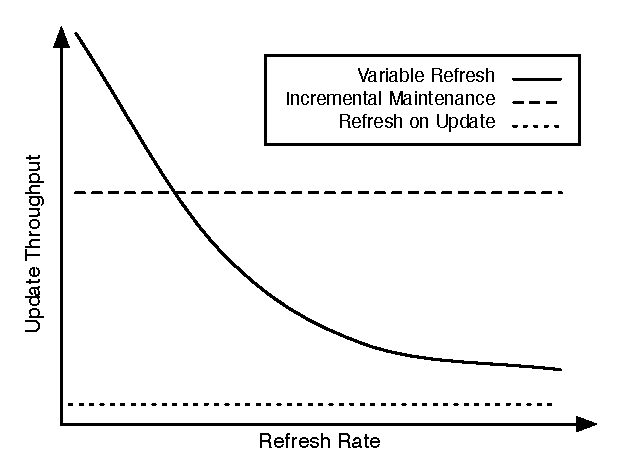
\includegraphics[width=2in]{../graphics-tmp/placeholder_db_result} &
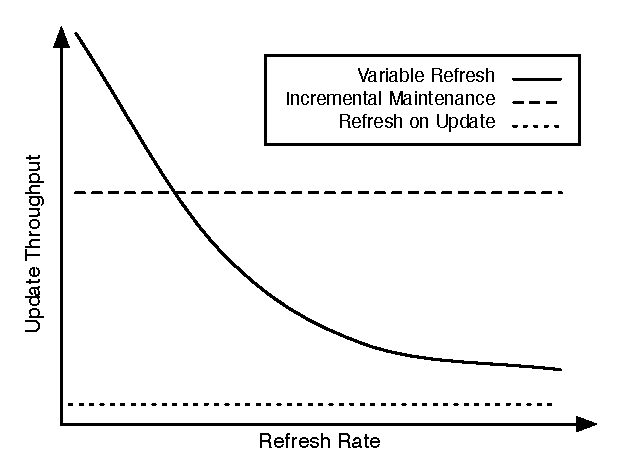
\includegraphics[width=2in]{../graphics-tmp/placeholder_db_result} &
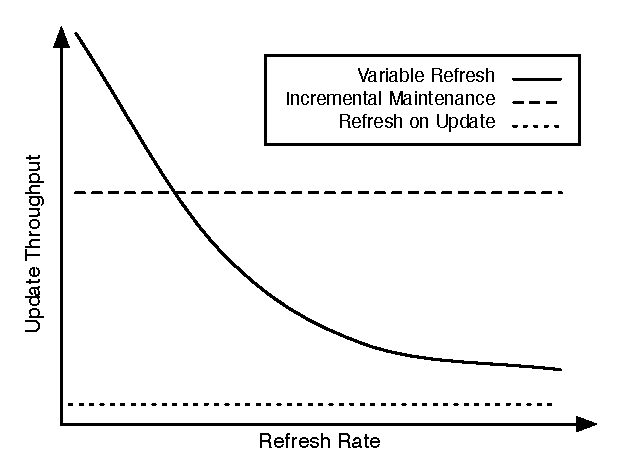
\includegraphics[width=2in]{../graphics-tmp/placeholder_db_result} \\
(a) & (b) & (c)
\end{tabular}
\end{center}
\label{fig:dbfail:postgres}
\caption{Performance results for Postgres on Examples \ref{ex:dbfail:stock} (a), \ref{ex:dbfail:tpch} (b), and \ref{ex:dbfail:network} (c).}
\end{figure*}
\begin{figure*}
\begin{center}
\begin{tabular}{ccc}
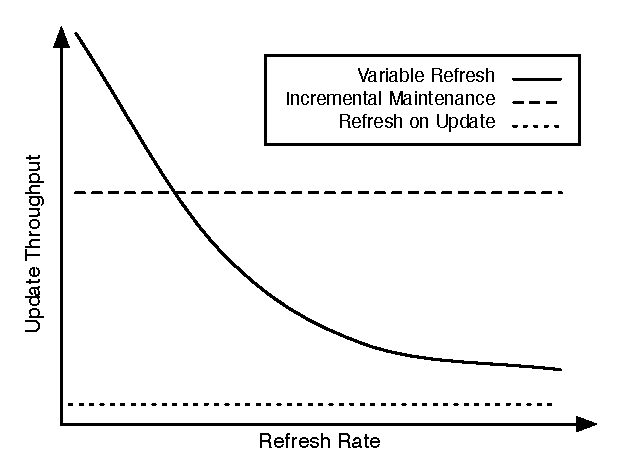
\includegraphics[width=2in]{../graphics-tmp/placeholder_db_result} &
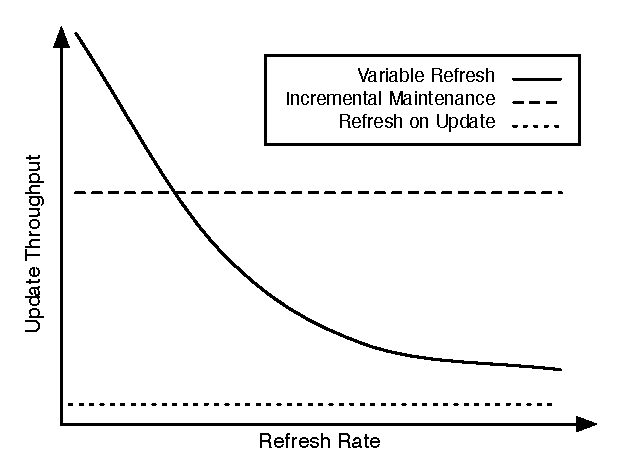
\includegraphics[width=2in]{../graphics-tmp/placeholder_db_result} &
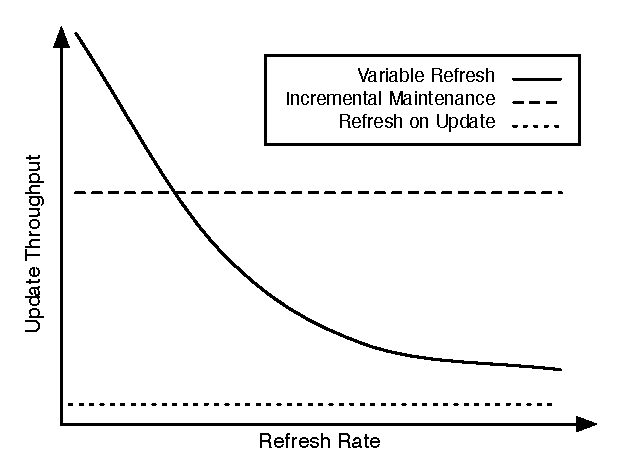
\includegraphics[width=2in]{../graphics-tmp/placeholder_db_result} \\
(a) & (b) & (c)
\end{tabular}
\end{center}
\label{fig:dbfail:CD1}
\caption{Performance results for Commercial DBMS 1 on Examples \ref{ex:dbfail:stock} (a), \ref{ex:dbfail:tpch} (b), and \ref{ex:dbfail:network} (c).}
\end{figure*}\begin{figure*}
\begin{center}
\begin{tabular}{ccc}
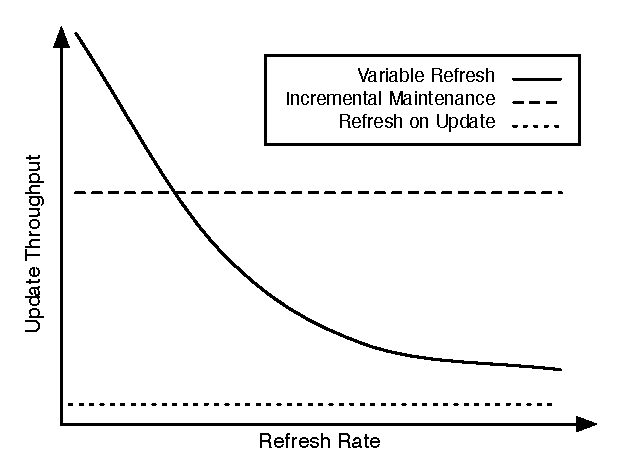
\includegraphics[width=2in]{../graphics-tmp/placeholder_db_result} &
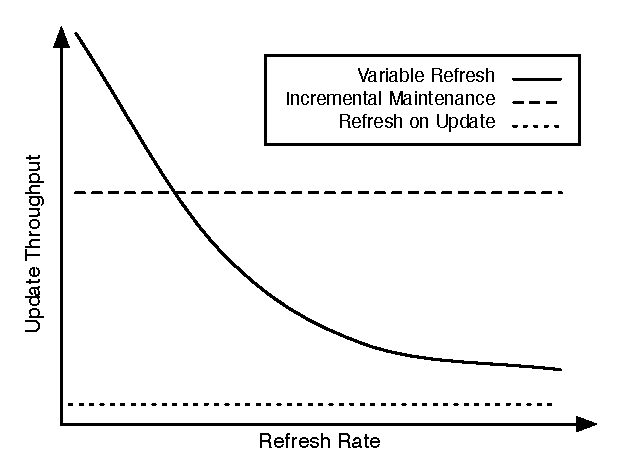
\includegraphics[width=2in]{../graphics-tmp/placeholder_db_result} &
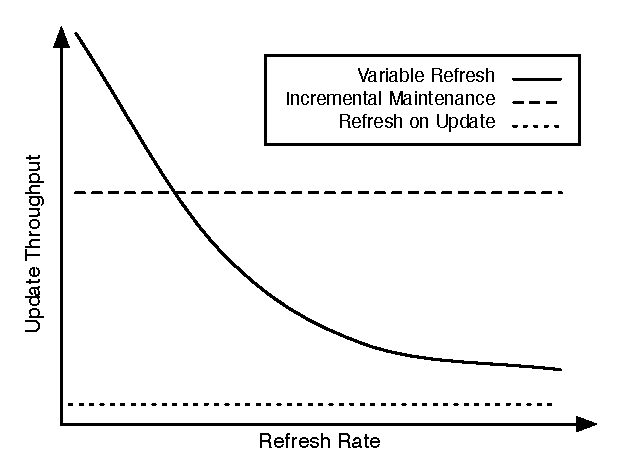
\includegraphics[width=2in]{../graphics-tmp/placeholder_db_result} \\
(a) & (b) & (c)
\end{tabular}
\end{center}
\label{fig:dbfail:CD2}
\caption{Performance results for Commercial DBMS 2 on Examples \ref{ex:dbfail:stock} (a), \ref{ex:dbfail:tpch} (b), and \ref{ex:dbfail:network} (c).}
\end{figure*}

Figures \ref{fig:dbfail:postgres}, \ref{fig:dbfail:CD1}, and \ref{fig:dbfail:CD2} show how the Postgres and two Commercial DBMSes (respectively) perform in each of the three example scenarios.  We consider three techniques for keeping a live view of the query result:
\begin{itemize}
\item {\bf Variable Refresh:} Periodically re-evaluate the query.  Note that in this implementation this results in the query not being monitored continually; The implementation can not detect trigger conditions which arise and disappear in between re-evaluations.
\item {\bf Full Refresh:} Use triggers to initiate a full refresh of the query results after every update to a base relation.  
\item {\bf Incremental Maintenance:} Use IVM to update the query results after every update to the base relation.  In the case of Postgres where IVM is not natively supported, we compute the delta query by hand and implement it via triggers.
\end{itemize}

\todo{Hardware overview goes here}.  Each graph shows the rate of updates supported by our configuration with respect to the frequency with which the query results are refreshed.  The Full Refresh and Incremental Maintenance implementations refresh the query results after every update, and are unaffected by the desired refresh rate.

\todo{Rewrite this paragraph after we have results}
Even with IVM techniques (which must be implemented by hand for Postgres), these systems can handle a maximum of \todo{fill in} updates per second to the base relations.  If users are willing resort to sampling as infrequently as once per one or ten seconds, it is possible to improve that to as much as \todo{fill in} or \todo{fill in} updates per second respectively.  Even with sampling, this is not sufficient to achieve the sorts of update rates required by our example applications.

\subsection{Monitoring with Stream Processors}
Section \ref{sec:dbfail:active} is perhaps a little unfair.  Although these systems are designed to efficiently process complex queries, even those that support incremental view maintenance are not designed to support rapidly changing data.  Rapidly changing data is the domain of stream processing systems \cite{abadi2003aurora,arvind2003stream,chandrasekaran2003telegraphcq,abadi2005design}.  In a Stream Processing system, users define pipelines similar to traditional query plans, except that each edge in the plan is a continuous stream of data.  Selection and projection operators are evaluated immediately.  Sliding Window Operators\cite{datar2002maintaining} {\em temporarily} store tuples appearing on a stream, and allow joins over the most recent set of tuples.  

Although sliding window operators make it easier for a stream processor to provide realtime performance guarantees, relying exclusively on the sliding window operator precludes the use of persistent state.  Recently, most commercial stream processing systems have added support for hybrid queries over both streaming and static data -- an approach commonly referred to as Complex Event Processing (CEP)\cite{DBLP:conf/sigmod/WuDR06}.   

\begin{figure*}
\begin{center}
\begin{tabular}{ccc}
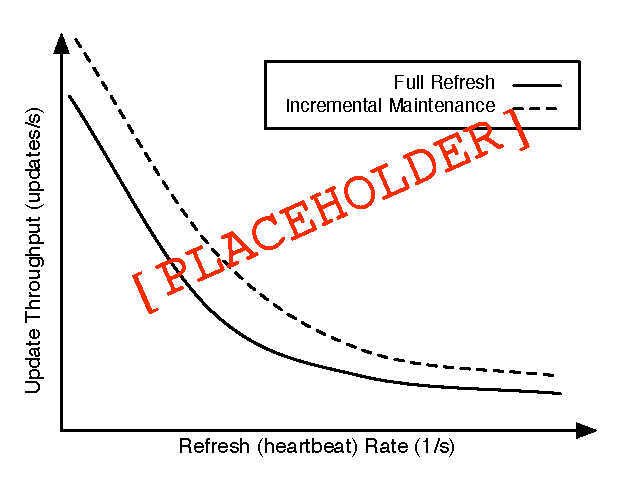
\includegraphics[width=2in]{../graphics-tmp/placeholder_stream_result} &
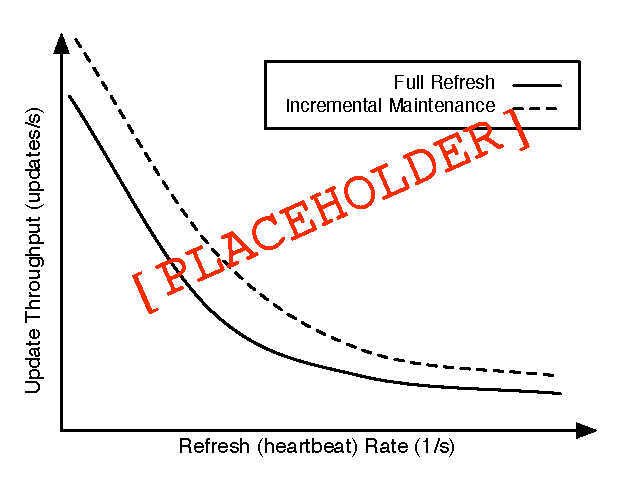
\includegraphics[width=2in]{../graphics-tmp/placeholder_stream_result} &
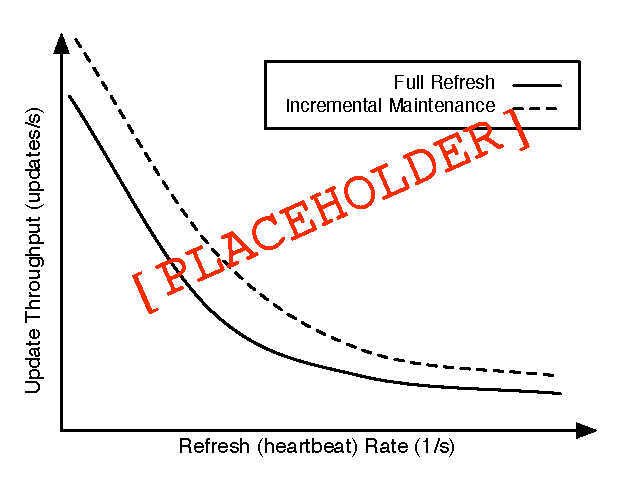
\includegraphics[width=2in]{../graphics-tmp/placeholder_stream_result} \\
(a) & (b) & (c)
\end{tabular}
\end{center}
\label{fig:dbfail:CSP1}
\caption{Performance results for Commercial Stream Processor 1 on Examples \ref{ex:dbfail:stock} (a), \ref{ex:dbfail:tpch} (b), and \ref{ex:dbfail:network} (c).}
\end{figure*}\begin{figure*}
\begin{center}
\begin{tabular}{ccc}
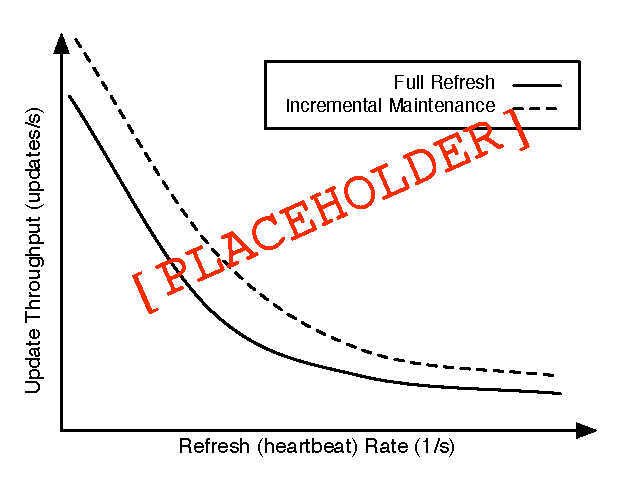
\includegraphics[width=2in]{../graphics-tmp/placeholder_stream_result} &
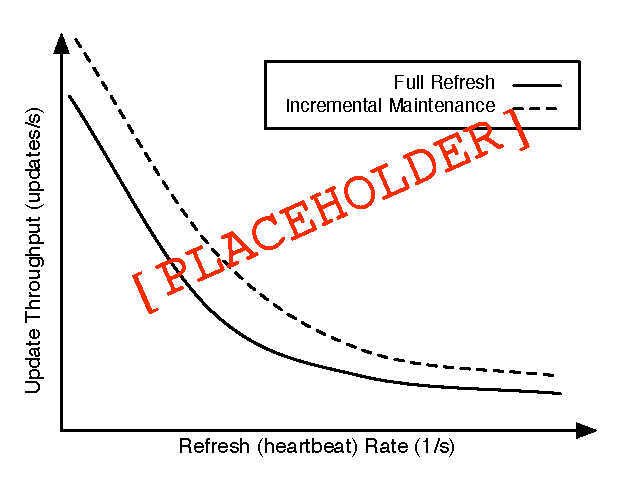
\includegraphics[width=2in]{../graphics-tmp/placeholder_stream_result} &
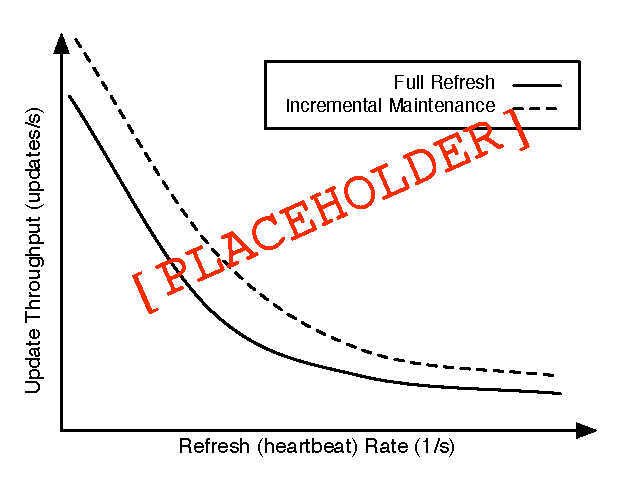
\includegraphics[width=2in]{../graphics-tmp/placeholder_stream_result} \\
(a) & (b) & (c)
\end{tabular}
\end{center}
\label{fig:dbfail:CSP2}
\caption{Performance results for Commercial Stream Processor 2 on Examples \ref{ex:dbfail:stock} (a), \ref{ex:dbfail:tpch} (b), and \ref{ex:dbfail:network} (c).}
\end{figure*}

Figures \ref{fig:dbfail:CSP1}, \ref{fig:dbfail:CSP2}, and \ref{fig:dbfail:CD2} show how two Commercial Stream Processing Systems perform in each of the three example scenarios.  We have also considered a third system, but were unable to implement these scenarios using it.

We consider two implementations of each example in each stream processor: one based on a straight translation of the query into the stream processor's language (Full Refresh), and one based on a translation of the delta queries that would have been generated by IVM (Incremental Maintenance) -- the delta queries are constructed by hand.

\todo{Rewrite this paragraph after we have results}
Even with IVM techniques (which must be implemented by hand in some implementations), these systems can handle a maximum of \todo{fill in} updates per second to the base relations.  This is, in part, the result of a need to lock the base relations before applying updates.  The CEP implementation in the stream processing systems we have analyzed is geared towards implementing tables as purely input or output sources -- persistent state used by the query is assumed to be relatively stable.  

\begin{figure}
\begin{center}
\begin{tabular}{|l|c|c|c|}
\hline
{\bf Engine}   & {\bf 2.1} & {\bf 2.2} & {\bf 2.3} \\\hline
{\bf Postgres} & 8 / 30    & 30 / 120  & 15 / 100 \\\hline
{\bf CDBMS 1}  & 8 / 9     & 30 / 31   & 15 / 16  \\\hline
{\bf CDBMS 2}  & 8 / 9     & 30 / 31   & 15 / 16  \\\hline
{\bf CSP 1}    & 40 / 120  & 60 / 200  & 50 / 200 \\\hline
{\bf CSP 2}    & 40 / 120  & 60 / 200  & 50 / 200 \\\hline
\end{tabular}

\todo{Update these numbers to be correct}
\end{center}
\label{fig:dbfail:locBakeoff}
\caption{Lines of code required to implement each of the example scenarios (including schema definitions) in Postgres, the two commercial database systems (CDBMS 1,2), and the two commercial stream processors (CSP 1,2).  For each engine/scenario pair, both the number of lines to implement the query and it's IVM equivalent are shown (respectively).}
\end{figure}

Another metric that must be considered is implementation complexity.  Figure \ref{fig:dbfail:locBakeoff} shows the number of lines of code required to implement each query in each of these engines.  The use of persistent state in the commercial stream processor forces the user to explicitly manage several messy aspects of the computation (e.g., locking the tables before updating/reading them).  Furthermore, when implementing IVM in systems that do not support it (Postgres and the two stream processors), the delta queries must be computed by hand and explicitly defined, causing a further blowup in number of lines.

\subsection{Implementation Challenges}
\todo{Yanif's horror stories}

\subsection{Other Related Work}
\comment{
In a database system, views are one of the central features in attaining both
logical data independence and efficient performance as evidenced by their use
from query optimization to data integration~\cite{halevy-vldbj01}. While
advances in view maintenance would have a significant impact on many database
internals challenges, our form of multilevel views and its realization as
efficient low-level code allows us to provide high-performance, lightweight
monitoring and notification services to the benefit of a wide range of
application domains. Consider the following applications:
}

Multilevel IVM
facilitates high-performance, lightweight monitoring for a wide range of
applications. Consider the following uses:

\vspace{-2mm}
\begin{list}{\labelenumi}{\usecounter{enumi} \leftmargin=1em}
\addtolength{\itemsep}{-0.5\baselineskip}
\item An automated stock market trading system monitors the distribution of buy
and sell orders of a particular stock to identify the best time and price for
its own orders.

\item A corporate data warehouse monitors its production facilities, warehoused
inventory and active demand for its products in order to identify
supply chain problems.

\item A compute cluster monitors its status to detect hardware failures
that place distributed tasks at risk of downtime.
\end{list}

\vspace{-1mm}
These uses require frontend analysis systems to drive rapid decision-making in
contrast to backend data warehouses for deep exploratory querying. These systems
sit on the critical datapath near data sources, and handle long-running,
machine-generated query workloads that require incremental evaluation, and
aggressive specialization during execution. While the need for
high-performance monitoring and view refresh is abundantly clear in algorithmic
trading, advertising, security and disaster prediction~\cite{scholz1973earthquake},
timely response is emerging as an essential ingredient of competitive advantage
and operational efficiencies in business, and service-oriented applications, and
benefits other domains such as regulatory compliance~\cite{basel2} and
scientific simulations~\cite{hey2009fourth}. To the best of our knowledge, no
data management systems have focused on extremely efficient continuous analysis
of large datasets that change in small high-impact increments.


\vspace{1mm}
\tinysection{Query Workloads for Monitoring}
The above scenarios of algorithmic trading on order books, online
decision support at a manufacturer, and datacenter and network infrastructure
monitoring often involve computing a variety of statistics,
and comparing and contrasting them prior to taking action.
\comment{
Queries with complex dataflows consisting of nested and correlated subqueries
composed in arbitrary fashion abound.
}
Figure~\ref{fig:queries} lists the processing properties of a query workload
inspired by these domains that we use in this paper, with SQL code in
Appendix~\ref{app:queries}.

The algorithmic trading queries operate on two order book streams of a day's
worth of orders for the MSFT symbol on NASDAQ (approx. 2.5 million orders). The
online decision support queries are taken from the TPC-H and SSB benchmarks, and
processed over a randomized, replayed update stream.
\comment{The cluster monitoring query operates on a synthetic dataset that
simulates tasks running on a 20,000 node cluster.}
Our workload has a range of joins, predicates, and correlated
subqueries, up to depth 2. While a depth of 2 may seem low, we have not seen
many queries in popular DBMS benchmarks even approaching 4 or 5 nesting levels.

\begin{figure}[t]
\scriptsize{
\begin{center}
\begin{tabular}{ p{0.15cm} | l | c | c | c  | c }
\multicolumn{2}{c|}{}      & \#~Tables,  & Where- & Group- & \#~Subqueries\\
\multicolumn{2}{c|}{}      & join type.  & clause & bys    & and depth\\
\multicolumn{2}{c|}{Query} & =: equi     &        &        & \\
\multicolumn{2}{c|}{}      & x: cross    &        &        & \\
\hline
\begin{rotate}{90}\hspace{-1.1cm}Finance\end{rotate}
& AXF        & 2, =      & $\vee, <$     & yes & 0 / 0 \\
& BSP        & 2, =      & $\wedge, <$   & yes & 0 / 0 \\
& BSV        & 2, =      & None          & no  & 0 / 0 \\
& MST        & 2, x      & $\wedge, <$   & yes & 2 / 1 \\
& PSP        & 2, x      & $\wedge, <$   & no  & 2 / 1 \\
& VWAP       & 1         & $<$           & no  & 2 / 1
\vspace{0.5mm}
\\
\hline
\begin{rotate}{90}\hspace{-0.9cm}ETL\end{rotate}
& TPCH3      & 3, =      & $\wedge, <$   & yes & 0 / 0 \\
& TPCH11     & 2, =      & None          & yes & 0 / 0 \\
& TPCH17     & 2, =      & $<$           & no  & 1 / 1 \\
& TPCH18     & 3, =      & $<$           & yes & 1 / 2 \\
& TPCH22     & 1         & $=,<$         & yes & 2 / 1 \\
& SSB4       & 7, =      & $<$           & yes & 0 / 0 \\
\hline
\comment{
& SVL        & 1         & $\wedge, <$   & yes & 2 / 1 \\
}
\end{tabular}
\end{center}
}
\vspace{-4mm}
\caption{Features of the algorithmic trading, online decision support, and
cluster monitoring query workload used for experiments.}
\label{fig:queries}
\vspace{-3mm}
\end{figure}

The pertinent DBMS methods are triggers, and stream systems.
We benchmarked these queries on a mix of open-source and commercial stream
systems and DBMS (Esper, Postgres, CSPE, CDB)\footnote{We anonymize the
commercial systems due to licensing restrictions on publishing benchmarks.},
Figure~\ref{fig:enginecomp} shows their view refresh performance.
\comment{  
We describe implementation specifics below but defer further details such as
system configuration, to our in-depth experiments in
Section~\ref{sec:experiments}.
}
We do not include any native IVM results from commercial DBMS because despite
its wide availability, there are still many limitations on its usability.
In fact, none of the major DBMS supported incremental refresh for the
majority of our workload given the features in Figure~\ref{fig:queries}.
For many DBMS, the documented query
restrictions~\cite{db2-viewrestrict,mssql-viewrestrict,oracle-viewrestrict}
indicate that view materialization and maintenance cannot generally be applied
side-by-side with query optimization.
\comment{
This is a strong motivator for our goal of including materialization as a
first-class citizen in query optimization.
}

\vspace{1mm}
\tinysection{Triggers and Active Databases}
Trigger mechanisms facilitate the manipulation of database state in a reactive
manner, as DML statements execute.
The literature on triggers has focused on issues such as cascading, and
recursion, and to a lesser extent single-level IVM~\cite{baralis-rids95}.
Triggers can be implemented in a variety of languages from plpgsql, to Python or
C. For procedural SQL languages, triggers are compiled in the same way as
user-defined queries for interpretation by an executor.
\comment{
Triggers exemplify update processing where the developer looses the ability for
declarative development, and where along with user-defined functions and
aggregates, compilers and query optimizers reside in silos inside a DBMS.
}
This executor is designed for set-at-a-time computation rather than
fine-grained, pipelined computation. 

We implemented a \textit{repetitive} full refresh approach to maintain views for
our query workload, where after each update a trigger re-evaluates the query
from scratch.
\comment{
This approach incurs low developer overhead. Manually implementing
multilevel view maintenance is rapidly impractical after even one level of delta
rewriting due to code expansion, affirming the benefits of automatic
incrementalization during compilation.
}
Figure~\ref{fig:enginecomp} shows that for the small-state finance workload,
trigger performance does not vary across the types of queries. Here small-state
refers to the state accumulated while processing updates. In the finance
workload there are nearly as many deletes as inserts (unsuccessful orders are
often removed from the order books), and relations do not grow too large. For
large-state workloads, on Postgres, queries with nesting perform signficantly
worse than on CDB. Overall, CDB performs the best across all engines, primarily
with the mature optimizer in CDB choosing better plans and index usage.

\begin{figure}[t]
\vspace{-1mm}
\begin{center}
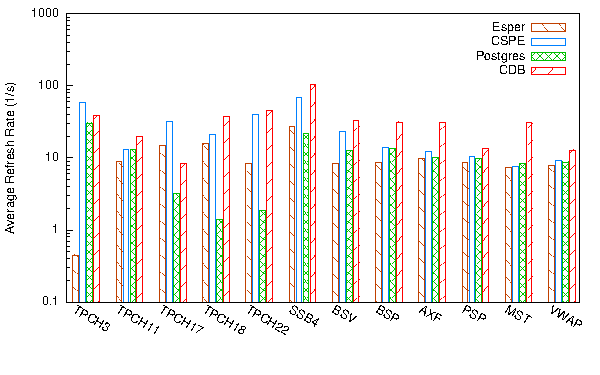
\includegraphics[scale=0.85]{../graphs/graphs/engine_bakeoff.pdf}
\end{center}
\vspace{-8mm}
\caption{A comparison of four stream systems and DBMS on full refresh view
maintenance.}
\label{fig:enginecomp}
\vspace{-4mm}
\end{figure}


\vspace{1mm}
\tinysection{Stream and Complex Event Processing}
These systems (SPEs) provide low-latency push-based processing and at first
glance may appear to be ideal for frontend analytics.
\comment{
However, in addition to
constructs such as windows or patterns and Kleene closure, monitoring
applications often have additional requirements -- they must often work with
long-lived, large state. This latter requirement is not well-addressed by
current SPEs, they rely on in-memory tables with suboptimal querying or
external DBMS access, and cannot support end-to-end incremental computation.
}
However, monitoring applications must often work with long-lived, large state,
and this requirement is not well-addressed by current SPEs. They either rely on
in-memory tables with suboptimal engines or external DBMS access, and do not
support incremental computation over large state.

Our implementation varied significantly across Esper and CSPE, due to a
clear lack of standardized semantics and portability across
SPEs~\cite{botan-pvldb:10,jain-pvldb:08}.
In both Esper and CSPE, we maintained indexed in-memory tables to represent base
relations, due to the inapplicability of windows to handle arbitrary updates and
deletes.
For Esper, we were unable to use subqueries in stream-to-table join operations,
which despite being supported in the language, resulted in differing,
inconsistent snapshots of tables that were used multiple times in a query (e.g.
self-joins), similar in effect to the state bug from
views~\cite{colby-sigmod:96}.
CSPE on the other hand did not support subqueries in stream-to-table operations.

On both systems, our approach performed stream-to-table joins to trigger the
replay of tables as streams via scans, as updates arrive. The replayed tables
were then processed by stream-only operators to implement fully pipelined plans.
\comment{
Our implementation strategy involved maintaining update streams as in-memory
tables, replaying relevant tables as updates arrive to turn tables into streams,
and wiring together stream operators to implement query plans. This essentially
constructs fully pipelined physical query plans and turns out to be very similar
to writing trigger code in procedural SQL languages once the stream is fully
replayed.
}
Additionally, we explicitly restricted both Esper and CSPE to single-threaded
execution and relied on their deterministic tuple processing order to avoid
complex locking and barriering to implement aggregate subqueries. We found such
serialization added substantial programming complexity and performance overheads
to our implementation.

Figure~\ref{fig:enginecomp} shows that for the finance workload, there is little
variation between Esper and CSPE, although CSPE does consistently outperform
Esper, but cannot match triggers in CDB. For the large-state queries, CSPE
outperforms Esper by significantly, and provides a viable alternative to
triggers in CDB with an overall lower variance in performance across both
nested (TPCH 17, 18, 22) and flat queries. Esper performs poorly on
TPCH 3 by missing index usage.
\comment{
Overall across all engines, we observed that index maintenance helped
significantly on the TPCH queries for a marginal maintenance cost.
}

The takeaway from these experiments is that with complex analysis workloads
involving nested queries and aggregate comparisons, SPEs often cannot take
advantage of the semantics they were designed for (e.g. windows, patterns), and
do not offer advantages over trigger processing. Furthermore neither system
achieves a high absolute refresh rate, of more than roughly 100 refreshes a
second suggesting limited responsiveness and poor scaling when considering many
simultaneous queries.

\tinysection{Other related work} In addition to the citations throughout this
paper, IBM's SPADE language~\cite{gedik-sigmod:08} has explored compilation and
fusion for stream queries, and Ghanem et
al.~\cite{DBLP:journals/tods/GhanemELA10} have presented a model for stream
processing with views. Neither of these consider as
general an incremental evaluation framework as multilevel views.


\section{The Compiler}
\label{sec:compiler}


In this section we present our compiler. We start by sketching its architecture.

The compiler accepts an SQL query and schema definition (essentially create table statements for the relations the query accesses) as input. The parser turns the input query into a first intermediate representation (IR) that is somewhat reminiscent of relational algebra. The first compilation stage generates trigger programs for performing multilevel incremental view maintenance (IVM). The statements of these trigger programs increment the values of view data structures (called maps) by expressions of this IR. The IR and basics of the transformation are described in Section~\ref{sec:compiler_calc}. Section~\ref{sec:simplification} presents optimizations for simplifying IRs in the first compilation stage.

In Section~\ref{sec:advanced-rewriting} we discuss the creation of triggers for multi-level incremental view maintenance by extracting and materializing strict subexpressions rather than the full query. This is necessary to be able to deal with nested aggregation which otherwise, if we always materialize the largest query we can, leads to recursion in compilation that does not terminate. In general, the choice of subquery to materialize and incrementally maintain is a degree of freedom in query optimization. In this section we give heuristic rules for making this choice.

The next stage of the compiler, described in Section~\ref{sec:kthree}, turns the statements of the trigger program created in the first stage into an IR for purely functional programming, essentially lambda calculus without general recursion but with special higher-order functions for transforming collections (primitives such as map and reduce). This stage allows us to perform deforestation and fusion optimizations too low-level to have expression in the first, relational algebra-like IR.
Section~\ref{sec:kthree} also describes our infrastructure for code generation and our runtime system.

TODO: show an architecture diagram.




\subsection{Queries with binding patterns, deltas, and recursive IVM}
\label{sec:compiler_calc}


\def\Sum{\mbox{Sum}}


Next we develop an IR for SQL queries that is suitable for compilation of database queries and to perform the transformations necessary to enable efficient multilevel IVM. This language is a refinement of the query language defined in \cite{koch-pods:10}, but here we aim at better readability and avoid unnecessary formality. The language is based on positive relational algebra with aggregation but makes the following modifications:
%
\begin{itemize}
\addtolength{\topsep}{-0.3ex}
\addtolength{\labelsep}{-0.3ex}
\addtolength{\itemsep}{-1ex}
\item
The data model is that of relations where tuples have {\em integer} multiplicities. This generalizes SQL bag semantics to allow for
negative multiplicities. This way, databases and updates can be treated uniformly. A relation in which all multiplicities are
nonnegative can be either thought of as an insertion or as a database (=an insertion into the empty database) and a relation in which all tuple multiplicities are negative is a deletion.

\item
We replace relational (bag) union by an operation $+$ that adds two relations $R$ and $S$ by assigning to each tuple in the result the integer sum of the multiplicities of that tuple in $R$ and $S$. The operation $+$ is associative, and this is key to the overall simplicity of the
approach and allows us to treat insertions and deletions uniformly.

\item
The join operation is the natural join, where the multiplicity of a tuple in the result
is the integer product of the multiplicities of the two tuples from which is formed.

\item
Conditions are queries in their own right; there is no explicit selection operation. Thus, we write a relational algebra selection
$\sigma_{A<B}(R)$ as $R \bowtie (A<B)$.

\item
Sum-aggregates are of the form $\Sum_{\vec{A}} Q$ where $Q$ is a query and $\vec{A}$ is a tuple of group-by columns (which we will also
call variables). The result are the tuples of the projection of $Q$ on $\vec{A}$ and each tuple's multiplicity is the sum of the
multiplicities of the tuples that were projected down to it.

\item
There are terms as in SQL, who have a scalar rather than relation value. A sum-aggregate without grouping column evaluates to a term.

\item
Terms can be used as queries; in that case, they evaluate to the nullary tuple with multiplicity the value of the term.
Thus an SQL query ``select sum(A) from R'' can be written in our IR as $\Sum(R \bowtie A)$; thus we first multiply the value of $A$ into the multiplicity of each tuple and than sum up all these multiplicities.

\item
There are no explicit operations for projection and relational difference. A multiplicity-aware projection is implemented by
sum-aggregation and universal queries can be expressed by counting aggregation (a popular homework exercise in database courses). All SQL aggregate functions can be expressed using sums (counts), ratios of sums (avg),
and nested aggregates (min and max)\footnote{Here, the materialization of the nested subquery
nicely corresponds to the materialization any IVM technique has to carry out to find second-best values when a min or max value is deleted.}.
\end{itemize}

Let us recap: The language departs from relational bag algebra in essentially two ways; by having integer tuple multiplicities
to deal uniformly with insertions and deletions, and by {\em taking aggregate values out of the tuple} and putting them down into
the multiplicity. This has a very desirable consequence: Incremental computation is all about modifying multiplicities.
As we will see later, by keeping aggregate values in the multiplicities, delta processing for aggregates is vastly simplified.
Aggregate queries dominate analytical workloads and can greatly profit from incremental view maintenance. Thus it makes sense to optimize our IR for aggregate processing.




In summary, the abstract syntax of the IR is two-sorted (consisting of queries $q$ and terms $t$):
%
\begin{eqnarray*}
q &\mbox{:--}& R \mid t \theta t \mid t \mid q + q \mid q \bowtie q \mid \Sum_{\vec{A}}(q) \\
t &\mbox{:--}& c \mid A                 \mid t + t \mid t * t       \mid \Sum(q)
\end{eqnarray*}
Thus queries can be formed from relation names, atomic conditions, addition, natural join, and sum-aggregation.
Terms are formed from constants, variables/columns, addition, multiplication, and sum-aggregation without group-by.
Terms are queries returning the nullary relation in which
tuple $\tuple{}$ has as multiplicity the value of the term. We use $Q_1 - Q_2$ as syntactic sugar for $Q_1 + (-1)\bowtie Q_2$.
Apart from this, the semantics was given above.


We will often use SQL syntax for conciseness, which will correspond to our IR in the natural way analogous to how we translate
between classical bag relational algebra and SQL.

Expressions of the IR have binding patterns: There are input variables or parameters
without which we cannot evaluate these expressions, and there are output variables, the columns of the schema of the query result.
%
Each expression $Q$ has input variables or parameters $\vec{x_{in}}$ and a set of output variables $\vec{x_{out}}$, which form the schema of the query result. We denote such an expression as $Q[\vec{x_{in}}][\vec{x_{out}}]$. The input variables are those that are not {\em range-restricted} in a calculus formulation, or equivalently have to be understood as {\em parameters} in a SQL query because their values cannot be computed from the database: They have to be provided so that the query can be evaluated.

Binding patterns represent information flow. In general, this flow is not exclusively bottom-up.
Some of an expression's variables are input variables or parameters which cannot be computed from the query but have to be given to the query so that it can be evaluated. The most interesting case of this is a correlated nested aggregate, viewed in isolation (which must be possible for small-step compositionality). In such an aggregate, the correlation variable from the outside is such an input variable. The aggregate query can only be computed if a value for the input variable is given.


We illustrate this by a few examples in Table~\ref{tab:ir-examples}.
All of the expressions there are valid queries of our IR, typed by indicating the input and output variables.

\begin{table}
\begin{center}
\begin{scriptsize}
\begin{tabular}{|l|l|l|}
\hline
SQL & IR & Bdg.pat. \\
\hline
select * from R   & $R$ & $[][A,B]$ \\
--- & $C < D$ & $[C,D][]$ \\
--- & $C = D$ & $[C][D]$ \\
&& or $[D][C]$
\\[1ex]
select A from R   & $\Sum_A(R \bowtie (B < C))$ & $[C][A]$ \\
where B < C       &&
\\[1ex]
select A, sum(1) from R  & $\Sum_A(R \bowtie (B < C))$ & $[C][A]$ \\
where B < C group by A &&
\\[1ex]
B < (select sum(D) from S & $B < \Sum(S \bowtie D$ & $[A,B][]$ \\
~~where A > C) & ~~$\bowtie (A > C))$ &
\\[1ex]
select * from R where & $\Sum_{A,B}(R \; \bowtie$ & $[][A,B]$ \\
B < (select sum(D) from S & ~~~~$B < \Sum(S \bowtie D$ & \\
where A > C) & ~~~~~~$\bowtie\; (A > C)))$ & \\
\hline
\end{tabular}
\end{scriptsize}
\end{center}

\vspace{-5mm}

\caption{Example queries with their binding patterns (written as [input vars][output vars]). Relation $R$ and S have schema $A,B$ and $C,D$, respectively.}
\label{tab:ir-examples}
\end{table}


\medskip



This language specification covers all of the core features of SQL with the exception of
null values and outer joins (which have the undesirably property of being nonassociative, which is a problem for incremental computation).



\subsubsection{Computing the delta of a query.}

This language has the nice property of being {\em closed under taking deltas}.
For each query expression $Q$, there
is an expression $\Delta Q$ of our IR that expresses how the result of $Q$ changes as the database $D$ is changed by update workload $\Delta D$. This works for updates containing an unbounded number of insertions and deletions, but we will subsequently only study single-tuple inserts and deletes.
The reason for this is that such updates allow for particularly efficient view refresh code that
can be run to respond online to each tuple change.


Thanks to the strong compositionality of the language, we only have to give delta rules for the 
individual operators. These rules a given and studied in detail in \cite{koch-pods:10}. In short,
\begin{eqnarray*}
\Delta(Q_1 + Q_2)    &:=& (\Delta Q_1) + (\Delta Q_2), \\ 
\Delta(\mbox{Sum } Q)   &:=& \mbox{Sum } (\Delta Q), \\
\Delta(Q_1 \bowtie Q_2) &:=& ((\Delta Q_1) \bowtie Q_2) + (Q_1 \bowtie (\Delta Q_2)) \\
&& +\; ((\Delta Q_1) \bowtie (\Delta Q_2)).
\end{eqnarray*}
$\Delta R$ is the update to $R$. In the case that the update does not change $R$ (but other relation(s)),
$\Delta R$ is empty.
 

The deltas of conditions are 0 if they do not contain nested queries. The delta for a condition with a nested query
is more complicated. For example, our rule for $\Delta (x > Q)$ is
$(x > (Q + \Delta Q)) \bowtie (x \le Q) - (x \le (Q + \Delta Q)) \bowtie (x > Q)$.
We refer to \cite{koch-pods:10} for the general case of conditions.

Let us be precise though about computing delta queries. In general, each expression has input and output variables,
and taking a delta in general {\em adds variables} parameterizing the query with the update. From now on we only consider single-tuple insertions $+R(\vec{x})$ to or deletions $-R(\vec{x})$ from a relation $R$.

\def\dxy{\Delta_{+R(x,y)}}

\begin{example}\em
\label{ex:RS}
Given schema $R(AB), S(CD)$, and query
\begin{verbatim}
select sum(A * D) from R, S where B < C
\end{verbatim}
or, in our IR,
$\Sum(R \bowtie S \bowtie B < C \bowtie A*D)[][]$.

The delta for this query and the insertion of a tuple $\tuple{x,y}$ into $R$ is as follows.
Let $e$ be $S \bowtie B < C \bowtie A*D$.
Then
\[
\dxy \Sum(R \bowtie e) = \Sum \dxy (R \bowtie e)
\]
and by the delta rule for $\bowtie$,
\begin{eqnarray*}
\dxy (R \bowtie e) &=& (\dxy R) \bowtie e \\
&+& R \bowtie \dxy e \\
&+& (\dxy R) \bowtie \dxy e
\end{eqnarray*}
%
and
$\dxy(e) = 0$
since
$\dxy S = 0$, $\dxy B \theta C = 0$, and $\dxy (A * D) = 0$. (This follows again from the delta rule for $\bowtie$, applied
twice.)
Now
$\dxy R$ is the singleton relation $\{\tuple{A:x,B:y}\}$: the actual insertion.
The expression $\{\tuple{A:x,B:y}\} \bowtie e$ can be simplified to
$\{\tuple{A:x}\} \bowtie S \bowtie y \theta C \bowtie x * D$.
%
Thus the delta of the input query is
$\Sum(\{\tuple{A:x}\} \bowtie  S \bowtie y < C \bowtie x*D)[x,y][]$ which can be further simplified to
$\Sum(S \bowtie y < C \bowtie x*D)[x,y][]$.
In SQL notation, this is
\begin{verbatim}
select sum(x * D) from S where y < C
\end{verbatim}
\end{example}




\subsubsection{Recursive incremental view maintenance.}

\def\deg{\mbox{deg}}

Before we come to multi-level IVM, let us recap the special case of recursive IVM of \cite{koch-pods:10, kennedy-ahmad-koch-cidr:11}, where we try to be as greedily incremental as possible.
If we restrict the query language to exclude aggregates nested into conditions (for which the delta query was complicated), the query language fragment has the following nice property \cite{koch-pods:10}.
%
$\Delta Q$ is structurally strictly simpler than $Q$ when query complexity is measured as follows. 
For union(+)-free queries, the {\em degree} $\deg(Q)$ of query $Q$ is the number of relations joined together. We can use distributivity to push unions above joins and so give a degree to queries with unions, as the maximum degree of the union-free subqueries. Queries are
strongly analogous to polynomials, and the degree of queries is defined precisely as it is defined for
polynomials.

\begin{theorem}[\cite{koch-pods:10}]
If $\deg(Q) > 0$, then \[\deg(\Delta Q) = \deg(Q) - 1.\]
\end{theorem}

Recursive IVM makes use of the simple fact that a delta query is a query too. Thus it can be incrementally maintained as well, making use of a delta query to the delta query, which again can be materialized and incrementally maintained, and so on, recursively.
By the above theorem, this recursive query transformation terminates in the $\deg(Q)$-th recursion level,
when the rewritten query becomes a ``constant'' (independent of the database, and only depending on the updates).

The goal of compilation is to create on-insert and on-delete triggers for every relation occurring in the query.
Conceptually, a query $Q[\vec{x}_{in}][\vec{x}_{out}]$ over relations $R_1, \dots, R_k$ is compiled as follows:
We write $M_Q$ for the materialized view of query $Q$. 
Then the trigger program for the event $\pm R_{i_{j+1}}(\vec{y}_{j+1})$ consists of the
statements

\begin{tabbing}
~~foreach $\vec{x}_{out}, \vec{y}_1, \dots, \vec{y}_j$ do \\
~~~~~
   $M_{\Delta_{\pm R_{i_j}} \dots \Delta_{\pm R_{i_1}} Q}
       [\vec{x}_{in}\vec{y}_1 \dots \vec{y}_j][\vec{x}_{out}] \;\pm=$ \\
~~~~~~~~
    $M_{\Delta_{\pm R_{i_{j+1}}} \dots \Delta_{\pm R_{i_1}} Q}
       [\vec{x}_{in}\vec{y}_1 \dots \vec{y}_{j+1}][\vec{x}_{out}]$.
\end{tabbing}
for each $j \in 0, 1, \dots, \deg(Q)$ and $\tuple{i_1 \dots i_j} \in 1, \dots, k^j$.
For correctness, unless we maintain
old and new versions of the maps (which would be costly), these statements have to be 
ordered by increasing $j$.

\begin{example}\em
\label{ex:RS2}
We return to the query $Q$ of Example~\ref{ex:RS}, and
$(\Delta_{\pm R(x,y)} Q)[x,y][]$ which was already computed there.
We compute:
\[ (\Delta_{\pm S(z,u)} Q)[z,u][] = \Sum(R \bowtie B < z \bowtie A*u) \]
and
\begin{eqnarray*}
(\Delta_{\pm S(z,u)} \Delta_{\pm R(x,y)} Q)[x,y,z,u][] &=& \\
(\Delta_{\pm R(x,y)} \Delta_{\pm S(z,u)} Q)[x,y,z,u][] &=&
\Sum(y < z \bowtie x*u) \\
&=& \mbox{$(y<z)$ ? $(x*u)$ : $0$}
\end{eqnarray*}
where $(y<z)$ ? $(x*u)$ : $0$ is the functional if-then-else of C
(if $y<z$ then $x*u$ else 0).
The on-insert into $R$ trigger $+R(x,y)$ following the construction described above is the program
\begin{tabbing}
$M_Q$[][] += $M_{\Delta_{+R(x,y)} Q}[x,y][]$; \\
foreach $z,u$ do $M_{\Delta_{+S(z,u)} Q}[z,u][]$ $+$= $(y<z)$ ? $(x*u)$ : $0$; \\
foreach $z,u$ do $M_{\Delta_{-S(z,u)} Q}[z,u][]$ $+$= $(y<z)$ ? $(x*u)$ : $0$
\end{tabbing}
The remaining triggers are constructed analogously.
The trigger contains an update rule for the (in this case, scalar) data structure $M_Q$ for the overall
query result, which uses the auxiliary view $M_{\Delta_{\pm R(x,y)} Q}$ which is maintained in the update triggers for $S$, plus update rules for the auxiliary views $M_{\Delta_{\pm S(z,u)} Q}$ that are used to update
$M_Q$ in the insertion and deletion triggers on updates to $S$.
\end{example}

We observe that the structure of the work that needs to be done is extremely regular and (conceptually) simple. Moreover,
there are no classical large-granularity operators left, so it does not make sense to give this workload to a classical
query optimizer. There are for-loops over many variables, which have the potential to be very expensive. But the work
is also perfectly data parallel, and there are no data dependencies comparable to those present in joins. All this provides
justification for adopting a compilers approach.


\subsubsection{Initial value computation}


The technique for constructing trigger programs by recursive delta rewriting discussed above assumes
materialized views to be represented as maps $M$ that store, for tuples $\vec{i}\vec{o}$ of input and output variables, a value (an aggregation result) $M[\vec{i}][\vec{o}]$.
So far we have disregarded the question what the {\em domains} of these maps are, that is,
for which $\vec{i}\vec{o}$ the maps are defined and store values.
If we could assume that the domains contain all the tuples that could ever be formed from values occurring
in the database, we could initialize the map values to zero, $M[\vec{i}][\vec{o}] := 0$,
before the first update is fed into the system.

However, it is not feasible to assume such large or even infinite domains.
Instead, we want to start with empty maps and extend the domains when the update triggers want to access
values -- for reading or writing -- that are not yet represented in the map.
This raises the question how to compute initialization values; in general, these will not be zero if 
the system has been running for a while and the maps contain data.
Take for instance the query of Example~\ref{ex:RS2}: Suppose so far we have only seen inserts into relation $R$,
but $S$ is still empty. Then the auxiliary maps $M_{\Delta_{+S(z,u)} Q}[z,u][]$ still have empty domains and
looping over each pair $\tuple{z,u}$ does nothing. When, later, a tuple $\tuple{z,u}$ is inserted into $S$,
$M_Q$ is incremented by $M_{\Delta_{+S(z,u)} Q}[z,u][]$, which has to be computed from scratch as
$\Sum(R \bowtie B < z \bowtie A*u)$ and will generally be nonzero.

In the currency system we use the fact that if a query defining does not use inequality joins, the map value
will be zero. Otherwise, the value is computed from scratch by executing the query that defines the map.
In the future, this could be improved upon by further compiling subqueries of this defining query using
recursive IVM techniques.


\subsection{Query decomposition and factorization}
\label{sec:simplification}


The construction for trigger programs presented above yields 
materializations of high dimensionality, which will be very large and so expensive to maintain.
This can be avoided by being slightly less aggressive with materialization.
We next discuss two query simplification techniques that are key to making
recursive incremental view maintenance useful, join graph decomposition and factorization
of query polynomials.


Join graph decomposition makes use of the so-called generalized distributive law [] (which plays
an important role in the context of probabilistic inference with graphical models) to decompose
sum-aggregates over disconnected join graphs. This is an important case, since computing deltas 
eliminates hyperedges of the join graph, disconnecting it more and more in each delta-rewriting, until all
hyperedges are gone. The basic law is simple. If a query is of the form $Q_1 \times Q_2$, i.e., $Q_1$ and
$Q_2$ do not share common columns, then
$\Sum_{\vec{A}\vec{B}}(Q_1 \times Q_2) = \Sum_{\vec{A}}(Q_2) \times \Sum{\vec{B}}(Q_2)$
where $\vec{A}$ are columns of $Q_1$ and $\vec{B}$ are columns of $Q_2.$
Consider for example the query $Q$
{\tt select sum(A*D) from R natural join S natural join T}
of schema $R(AB), S(BC), T(CDE)$. Then
$\Delta_{+S(b,c)} Q$ is
\begin{verbatim}
select sum(A*D) from R,T where B=b and C=c
   = (select sum(A) from R where B=b) *
     (select sum(D) from T where C=c)
\end{verbatim}
Given such a decomposition, it is better to materialize the two aggregate subexpressions and compute
the product when updating, rather than to materialize the product, that is,
\begin{eqnarray*}
M_Q[][] &+=& M_{\mathrm{select~sum(A)~from~R~where~B=b}}[b][] \\
&*& M_{\mathrm{select~sum(D)~from~T~where~C=C}}[c][]
\end{eqnarray*}
is better than
$M_Q[][] += M_{\Delta_{+S(b,c)} Q}[b,c][]$ because that way we materialize two (small) one-dimensional
maps rather than one two-dimensional map.

Binary sums  (unions) $+$ can be pushed through aggregate sums ($\Sum(Q_1 + Q_2) = \Sum(Q_1) + \Sum(Q_2)$).
In conjunction with join graph decomposition, this often leaves us with expressions that do a fair amount
of adding and multiplying of subqueries. Such expressions can be optimized using the distributive law.
Factorization is often particularly useful to share common subexpressions.
For example, the general delta rule for $Q_1 \bowtie Q_2$ is a sum of three subexpressions
$\Delta(Q_1 \bowtie Q_2) := ((\Delta Q_1) \bowtie Q_2) + (Q_1 \bowtie (\Delta Q_2))
 + ((\Delta Q_1) \bowtie (\Delta Q_2))$ which can be factorized as
$((Q_1 + \Delta Q_1) \bowtie (\Delta Q_2)) + ((\Delta Q_1) \bowtie  Q_2)$
or as
$((\Delta Q_1) \bowtie (Q_2 + \Delta Q_2)) + (Q_1 \bowtie \Delta Q_2)$.
Determining which one is better is a task for a cost-based optimizer.








\subsection{Inequality Joins and nested aggregation}
\label{sec:advanced-rewriting}

This subsection gives heuristics for choosing which subqueries of
a query to extract and materialize for incremental view maintenance.
The delta queries created according to the construction presented in
Section~\ref{sec:compiler_calc} can be made subject to the same optimization as well, but differently from the recursive
incremental view maintenance (IVM) method sketched above we do not have to always aggressively materialize the full query being analyzed.

This extract/materialize rewriting in its more general form remains useful in a compilation
approach (the code generated is however, less straightforward and may now
perform more complex computations), it is also useful as an optimization technique in more
classical query engines.

We have observed above that recursive IVM fails for queries with nested aggregate subqueries. However,
as we will see next, we can extract and materialize the subquery without its aggregation and performing the aggregation nonincrementally on top of the materialized view. That materialized view can be optimized further using multilevel incremental view maintenance.

Example: TODO


As a general heuristic, we want to evaluate nested aggregates and inequality joins nonincrementally, but can maintain their subexpressions incrementally. Inequality joins
require costly domain maintenance for cached values that are frequently not accessed again.
Materialization does not pay off for inequality joins for the code we are currently creating,
but in the future, this could change. We could employ a suitable garbage collection scheme that allows us to stop keeping multiplicities of tuples we do not expect to use again (soon) fresh and accurate. Another idea is to use
suitable data structures such as range trees rather than hash maps (TODO: this is a forward ref currently) to efficiently maintain materialized inequality joins.

TODO: Explain this by an example.

TODO: Do we have further insights and heuristics?


\subsection{Functional compilation and optimization}
\label{sec:kthree}



\def\map{\mbox{\texttt{map}}}
\def\flatten{\mbox{\texttt{flatten}}}
\def\agg{\mbox{\texttt{agg}}}
\def\groupagg{\mbox{\texttt{groupagg}}}
\def\apply{\mbox{\texttt{apply}}}


\comment{
Each step of delta transformation, and extraction and materialization
in our recursive compilation process results in a maintenance query with parameters
(i.e. a function) that updates an auxiliary datastructure. This leads to our
second stage IR, a small functional programming IR.
}
To narrow the gap while translating the SQL IR directly to low-level code, our
second stage IR is a small functional programming language.
\comment{
Functional programs have strong correspondences to relational queries, both are
dataflow programs, and the relationship of their formal expressiveness has been
studied in complex object languages~\cite{buneman-kleisli:95}, and
comprehensions~\cite{jones-haskell:07}.
}
We perform holistic query optimization in a functional IR, exploiting a
breadth of powerful program transformations including monad transformations from
structural recursion~\cite{buneman-kleisli:95},
deforestation~\cite{marlow-fp:92}, supercompilation and fusion.
Other recent works have observed the need for holistic optimization of query
executors with low-level languages~\cite{krikellas-icde:10,neumann-pvldb:11}.
Our functional IR is a work-in-progress that we believe will bring benefits such
as simpler optimizer development, and non-first normal forms for specialized
in-memory or disk layout strategies in future work.


Our functional IR includes tuples and collection types, lambdas and associative
lambdas\footnote{Determining properties such as associativity, commutativity and
idempotence via program analyses is undecidable~\cite{buneman-kleisli:95}},
conditionals, four higher-order collection transformers that we describe below,
and in-place update operations on collections.
\comment{
Collection mutation operations perform in-place updates of entries, implying
that our functional IR is an impure language, although we could use monads as
with Haskell's I/O system.
}
Also, our functions are not recursive, and only our collection transformers use
higher-order functions, that is we never pass a function as an argument to
another function. Our functional IR is already low-level in the spirit of
functional compiler internal IRs (i.e. after defunctionalization).



For our higher-order collection transformers, we extend the \texttt{map} and
\texttt{flatten} constructs from Kleisli~\cite{buneman-kleisli:95} with
aggregations: \texttt{agg} and \texttt{groupagg}. Their type signatures are:


\vspace{1mm}\hspace{-4mm}
\begin{tabular}{p{1cm}l}
\texttt{map}
    & $: (\sigma \rightarrow \tau)
           \rightarrow \sigma \ \mathcal{C}
           \rightarrow \tau \ \mathcal{C}$\\
\texttt{flatten}       
    & $: (\sigma\ \mathcal{C}) \ \mathcal{C}
           \rightarrow \sigma \ \mathcal{C}$ \\
\texttt{agg}
    & $: (\sigma \rightarrow \tau \rightarrow \tau)
           \rightarrow \tau
           \rightarrow \sigma \ \mathcal{C}
           \rightarrow \tau$ \\
\texttt{groupagg}
    & $: (\sigma \rightarrow \tau \rightarrow \tau)
           \rightarrow (\sigma \rightarrow \upsilon)
           \rightarrow \tau
           \rightarrow \sigma \ \mathcal{C}
           \rightarrow \tuple{\upsilon, \tau} \ \mathcal{C}$ \\
\end{tabular}

\comment{
Type signatures for our collection mutators are:

\vspace{1mm}
\begin{tabular}{p{0.8cm}l}
\texttt{merge}
    & $: \tuple{\sigma, \tau} \ \mathcal{C}
           \rightarrow \tuple{\sigma, \tau} \ \mathcal{C}
           \rightarrow \tuple{\sigma, \tau} \ \mathcal{C}$ \\
\texttt{update} 
    & $: \tuple{\sigma, \tau} \ \mathcal{C}
           \rightarrow \tuple{\sigma, \tau}
           \rightarrow \tuple{\sigma, \tau} \ \mathcal{C}$
\end{tabular}

\todo{Describe these operations}
}

\vspace{1mm}
\noindent Above $\sigma \ \mathcal{C}$ indicates the type of a collection
containing elements of type $\sigma$, and $\tuple{}$ is a tuple constructor. The
\texttt{map} transformer applies a function to every element of a collection,
while \texttt{flatten} reduces a two-level nested collection to a flat
collection. The \texttt{agg} and \texttt{groupagg} transformers applies the
accumulator function given as its first argument over a collection. Both are
given an initial value, and \texttt{groupagg} is additionally given a grouping
or partitioning function as its second argument. Our framework is agnostic to
the form of collection, which may be sets, bags, and lists, and
can vary in their underlying implementation (e.g. tree or hash sets, linked lists or
vectors). Intelligent datastructure selection is future work, we currently use
vectors and hashtables.

Our functional IR supports several optimizations that are not captured by the
SQL IR, including:
\comment{
Currently, our optimizer performs static compile-time optimizations that
universally simplify functional programs in its usage of collections and
scalars. We plan to expand this to perform both cost-based static and runtime
adaptive optimizations in future work.
}

\vspace{1mm}
\noindent\textbf{If-lifting.} This is a transformation to a canonical form
for our functional IR that involves lifting every conditional to its minimal
binding point. Consider an expression:

$\apply(\lambda x. \apply(\lambda y.
  \mbox{\texttt{ if }} x < 0 \mbox{\texttt{ then }} y/a
                             \mbox{\texttt{ else }} y*3, a), b)$

\vspace{1mm}
\noindent The conditional above is independent of $y$ and we can lift to:

\vspace{-2mm}
\begin{tabbing}
$\apply(\lambda x.
  \mbox{\texttt{ if }} x < 0$ \= $\mbox{\texttt{ then }}
    \apply(\lambda y. y/a, a)$\\
\> $\mbox{\texttt{ else }} \apply(\lambda y. y*3, a),\ b)$
\end{tabbing}


\vspace{-2mm}  
\comment{
A minimal binding point is the lambda expression that binds the minimal
sufficient set of variables to ensure a well-defined evaluation of the
conditional.
}
\noindent This canonical form admits maximal optimization of the conditional's
then-else blocks by pushing in expressions from outside the conditional
at the expense of code size. However, queries are often small
in code size, and if-lifting enables joint optimization of IVC expressions and
delta expressions.


\vspace{1mm}
\noindent\textbf{Deforestation and fusion.} This transformation converts
functional programs to treeless forms~\cite{marlow-fp:92}, that is, it eliminates
redundant intermediate datastructures. The core subset of our deforestation
rewrite rules are:

\def\xform{\mbox{\texttt{:-}}}
\def\fst{\mbox{\texttt{fst}}}

\vspace{1mm}\hspace{-6mm}
\begin{tabular}{p{3.6cm}l}
$\map(f, \map(f', c))$ 
    & $\xform\ \map(f \circ f', c)$
\\
$\map(f, \flatten(c))$
    & $\xform\ \flatten(\map(\lambda c'.\ \map(f,c'), c))$
\\
$\agg(f^a, i, \map(f', c))$
    & $\xform\ \agg(f^a \circ f', i, c)$
\\
$\agg(f^a, i, \flatten(c))$
    & $\xform\ \agg(f, i, \map(\lambda c'.\ \agg(f, i, c'),c))$
\\
$\groupagg(f^a, g, i, \map(f', c))$
    & $\xform\ \groupagg(f^a \circ f', g \circ f', i, c)$
\\
$\groupagg(f^a, i, \flatten(c))$ & $\xform$
\\
\multicolumn{2}{l}{
$\quad\groupagg(f, \fst, i, \flatten(
    \map(\lambda c'.\ \groupagg(f, g, i, c'),c)))$}
\end{tabular}


\vspace{1mm}
Above $\circ$ is function composition and \texttt{fst} the left projection of a
pair.
\comment{
Note that both the \texttt{agg} and \texttt{groupagg} compose
associative lambdas (above $f^a$, two-argument lambdas), with regular
(single-argument) lambdas in terms of the first argument.
}
Additional deforestation rules for iterative usage of in-place updates are
straightforward to derive.

The first rule for \texttt{map} eliminates the intermediate collection
constructed after applying $f'$, instead pipelining the results through the
application of both functions $f$ and $f'$. Since both $f$ and $f'$ can
themselves contain \texttt{map} invocations, essentially performing joins, this
rule can alter the arity of the join operation, constructing fully pipelined
n-way joins. The second rule above is a form of late tuple
construction~\cite{abadi-icde:07}, where by lifting the \texttt{flatten}
expression, we carry around nested intermediate collection during processing.
Repeating this facilitates deeply nested representations, in the same vein as
non-first normal forms~\cite{schek-infsys:86}. Aggregate deforestation also uses
composition to realize pipelining and simplification, and the variants with
\texttt{flatten} are partial aggregations that push an associative aggregation
inside a nested collection.

\comment{
\vspace{1mm}
\noindent\textbf{Other optimizations.} The other major simplifications that we
perform on our functional IR include common subexpression elimination and
initial value computation deduplication. Duplicate, redundant IVC arises in the
SQL IR since the same view can appear multiple times when taking deltas of sums
and products expressions. We omit full details of these due to space
restrictions.
}

\comment{
\vspace{1mm}
\noindent\textbf{Common subexpression elimination.}
Our CSE algorithm simultaneously extracts candidate common subexpressions and
substitutes their usage, prioritizing large expressions as candidates. Our
approach is conservative, candidates extracted from disjunctions and
conditionals must be candidates in all subexpressions, to avoid unnecessary
evaluation in light of short-circuiting on disjunctions and conditions. Our
substitution process considers expression equivalence under alpha renaming
rather than pure lexical comparison, as with global value numbering strategies.
\comment{
Currently our CSE algorithm operates separately on side-effecting queries, and
we plan to analyze all maintenance work performed to realize multi-query
optimization.
}

\vspace{1mm}
\noindent\textbf{IVC deduplication.} In the SQL IR, the same view can appear
multiple times when taking deltas of sums and products expressions. Subsequently
its initial value computation (IVC) will also appear many times and when
accounting for binding patterns, these initial value computations are idempotent
and redundant. We can eliminate duplicate IVCs by tracking of binding pattern
equivalences and their dependences on variable domains.
}

\comment{
\vspace{1mm}
\noindent\textbf{Datastructure creation.} The final optimization pass creates
auxiliary index datastructures to efficiently evaluate predicates. This stage
occurs last since the prior optimizations, with the exception of if-lifting,
yield a simpler and smaller functional IR. We presently implement hash
datastructures, by extracting any remaining equality predicates from the IR,
and synthesize an expression to construct a hashtable on-the-fly and perform
probes.
}


\noindent\textbf{Code generation} Following functional optimization, we
synthesize an imperative IR for easy code generation as the final step of
compilation.
\comment{
The synthesis process is extensible in that a code generator
developer can define additional materialization points for temporaries given
their target language since different backend languages have varying built-in
primitive operations and datastructures.
}
The imperative IR supports external functions and types to enable the usage
of library code. We implemented a C++ code generator based around the STL and
its iterator-oriented collection APIs (e.g. \texttt{begin}, \texttt{end},
\texttt{find}, \texttt{erase}, \texttt{clear}, etc.). We omit further details
due to space constraints. Our imperative optimizer and its datastructure and
storage layer concerns is a work-in-progress.



\section{Experimental Results}
\label{sec:experiments}

\newcommand{\figurewidth}[0]{1.8in}

\newcommand{\tablefig}[1]{
  \hspace*{-0.25in}
  \includegraphics[width=\figurewidth]{../graphs/graphs/#1}
}

\begin{figure}
\begin{center}
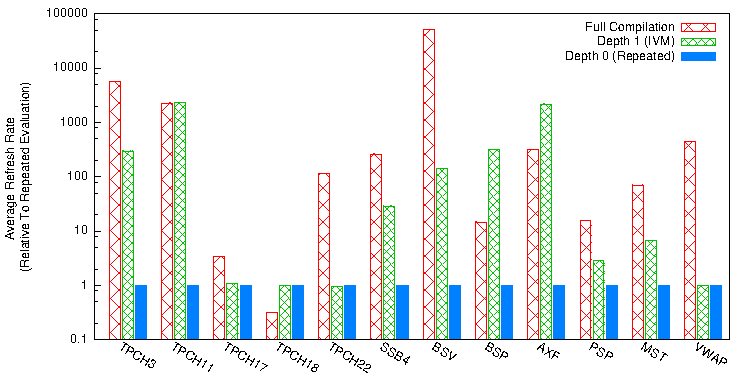
\includegraphics[width=3.4in]{../graphs/graphs/bakeoff.pdf}
\caption{Cross-query comparison of our compiler in different depth-restricted modes, and the best performing streaming and database engine for each query.  Note the logscale on the y-axis.}
\label{fig:experiments:bakeoff}
\end{center}
\end{figure}

\begin{figure*}
\begin{center}

\begin{minipage}{\textwidth}
\begin{center}
\hspace*{0.1in}
\begin{tabular}{cccc}
\tablefig{unified_tpch3.pdf} &
\tablefig{unified_tpch11.pdf} &
\tablefig{unified_tpch17.pdf} &
\tablefig{unified_ssb4.pdf} \\
(a) & (b) & (c) & (d)
\end{tabular}
\caption{TPC-H Query 3~(a), 11~(b), 17~(c), and SSB4~(d): (a) By the 40\%\ marker, all streams except LINEITEM have completed, and the remaining tuples consume no additional memory. (b) For simple two-way joins, full compilation is virtually identical to depth 1. (c) Due to the nested aggregate, IVC requires a nested loop, while full compilation requires only a single scan.(d) Full compilation is a full polynomial order faster than in IVC, although performance does begin to drop once the system begins running out of memory around the 27\%\ marker.}
\label{fig:experiments:tpch3}  
\label{fig:experiments:ssb4}
\label{fig:experiments:tpch17}
\label{fig:experiments:tpch11}
\end{center}
\end{minipage}

\vspace*{0.2in}

\begin{minipage}{\textwidth}
\hspace*{0.1in}
\begin{tabular}{cccc}
\tablefig{unified_brokervariance.pdf} & 
\tablefig{unified_tpch22.pdf} &
\tablefig{unified_vwap.pdf} &
\tablefig{unified_serverload.pdf} \\
(a) & (b) & (c) & (d)
\end{tabular}
\caption{BSV~(a), TPC-H Query 22~(b), VWAP~(c), and SVL~(d):  (a) The many-to-many relationship on the join term forces IVM to perform linear work on each insertion, which full compilation avoids.  (b) The small CUSTOMER stream completes at the 10\%\ marker, while the remaining ORDERS tuples require only linear time with full compilation. (c) IVM repeatedly re-evaluates the nested (parameterized) sub-query, while full compilation maintais a cache of sub-query results. (d) Materializing nested queries gains a polynomial degree of performance over IVM, but memory continues to grow. }
\label{fig:experiments:brokervariance}
\label{fig:experiments:tpch22}
\label{fig:experiments:vwap}
\label{fig:experiments:serverload}
\end{minipage}

\vspace*{0.2in}

\begin{minipage}{\textwidth}
\hspace*{0.1in}
\begin{tabular}{cccc}
\tablefig{unified_pricespread.pdf} &
\tablefig{unified_missedtrades.pdf} &
\tablefig{unified_axfinder.pdf} &
\tablefig{unified_brokerspread.pdf} \\
(a) & (b) & (c) & (d)
\end{tabular}
\caption{PS~(a), MST~(b), AXF~(c) and BSP~(d):  (a,b) The performance and memory plateaus result from a portion of the trace from about 0.001\%\ to 0.01\%, where a single order is repeatedly placed and revoked. (c,d) Full compilation's aggressive materialization strategy results in the caches growing too large to be efficiently maintained.}
\label{fig:experiments:pricespread}
\label{fig:experiments:MST}
\label{fig:experiments:axfinder}
\label{fig:experiments:brokerspread}
\end{minipage}



\end{center}
\end{figure*}

\begin{figure*}
\begin{center}

%\begin{minipage}{\textwidth}
%\begin{center}
%\begin{tabular}{ccc}
%(a) & (b) & (c)
%\end{tabular}
%\caption{TPC-H Query 18~(a). }
%\label{fig:experiments:tpch18}
%\end{center}
%\end{minipage}
%
\vspace*{0.1in}

\begin{minipage}{\textwidth}
\begin{center}
\begin{tabular}{cccc}
\tablefig{unified_tpch18.pdf} &
\tablefig{unified_5gig_tpch3.pdf} &
\tablefig{unified_5gig_tpch11.pdf} &
\tablefig{unified_5gig_tpch22.pdf} \\
(a) & (b) & (c) & (d)
\end{tabular}
\caption{TPCH Query 18 (a): An incorrectly chosen join ordering prevents full compilation from effectively exploiting foreign key dependencies in the TPC-H schema;  The three fastest-running TPC-H queries (3~(b), 11~(c), and 22~(d)) run on a 5GB dataset: (b) Quadratic effects from early parts of the workload become apparent in IVM at this scale, while full compilation remains linear. (c) Maintaining the base relations already projected and aggregated gives a slight edge to full compilation at this scale.  (d) Full compilation performance is reduced due to updates being linear in the size of CUSTOMER, but still performs better than depth 1.}
\label{fig:experiments:big}
\label{fig:experiments:big:tpch3}
\label{fig:experiments:big:tpch11}
\label{fig:experiments:big:tpch22}
\end{center}
\end{minipage}

\end{center}
\end{figure*}

We now analyze the performance of our compilation techniques.  As in Section \ref{sec:dbfail}, our experiments are run on Redhat Enterprise Linux running in a VM with 16 GB of RAM, and 2x4 core Intel Xeon E5620 2.4 GHz processors allocated to it.  Note that our compiler produces single-threaded code, while other platforms were allowed to consume the full resources of the VM.

Our analysis uses the same queries and methodology as in Section~\ref{sec:tscomparison}: The queries are described in Section~\ref{sec:tscomparison:workload}, and expressed in SQL form in Appendix~\ref{app:queries}.

% we analyze our compiler's performance on TPC-H\cite{tpch} Queries 3, 11, 17, 18, and 22, a variant of Star Schema Benchmark\cite{ssb} Query 4 six orderbook queries: VWAP, PS, MST, AXF, BSP, and BSV, and a cluster monitoring query: SVL.  TPC-H queries were modified slightly due to a lack of support for certain advanced features in our SQL parser (e.g., Having, Exists, etc...).  SQL for the queries in our test workload is presented in Appendix

%Our analysis uses the queries from Examples \ref{ex:dbfail:stock} (PS),  \ref{ex:dbfail:tpch} (SSB4), and \ref{ex:dbfail:network} (SVL), Queries numbers 3, 11, 17, 18, and 22 from the TPC-H\cite{tpch} benchmark, the VWAP query presented in \cite{kennedy-ahmad-koch-cidr:11}, and four additional financial queries: MST, AXF, BSP, and BSV in the spirit of VWAP and PS.  The structure of these queries is discussed below.

Queries were run on pre-generated traces until completion of the trace or a 1 hour cutoff was reached.  Traces were generated as follows: The queries: VWAP, MST, AXF, BSP, PS, and BSV were run on a 2.63 million tuple trace of an order book update stream, representing of one day of stock market activity for MSFT.  BID and ASK orders (and cancellations) were translated into equivalent operations on a BIDS and ASKS table, with tuples in either table comprised of a timestamp, an order id, a broker id, a price, and a volume.  The broker id was synthesized for each order -- our experiments use 10 brokers, assigned deterministically based on the order id.  The stream consists of approximately 1.4 million operations on the BIDS table, and 1.14 million operations on the ASKS table.

Queries based on the TPC-H schema (including SSB4) were run on a scaling-factor 0.1 (100 BM) database generated by dbgen\cite{tpch}.  Additional scaling experiments were carried out on TPC-H queries 3 and 11 at scaling factors 0.5, 1, 5, and 10 -- these results are presented in Section~\ref{sec:experiments:bigds}.  Insertions are drawn in-order from each output file of dbgen, with rows from different tables interleaved in random order.  Note that it possible for rows to be inserted before a foreign key constraint has been satisfied, and that smaller datafiles will finish earlier in the stream.  This is not expected behavior in a streaming setting, but provides valuable insights about the performance characteristics of insertions into different tables.

SVL was run on a synthetically generated dataset, simulating 1000 racks of 20 servers each, emitting a total of 100,000 state updates.  The first 20,000 operations in the trace consist of an insertion for each server at 0 load.  For each state update, a random server deletes its previous state tuple and inserts a tuple declaring its new load -- a random real between 0 and 1.

Figure \ref{fig:experiments:bakeoff} compares recursive compilation to the performance of traditional databases and stream processors -- results presented overlap with those of Figure~\ref{fig:queries}.  These numbers speak for themselves, but clearly, traditional engines are not designed for our problem domain.

In order to evaluate our compilation algorithm in a fair environment with a common baseline for performance, we use a depth-limited instantiation of our compilation algorithm: Instead of recursively computing the entire materialization plan, the compiler stops after a fixed number of recursive steps.  Beyond this stage, queries are not materialized and instead computed directly from the base relations.

Compilation at depth-1 is equivalent to traditional IVM techniques, and depth-0 is equivalent to re-evaluating the query on every insertion.  We omit detailed depth-0 performance measurements on graphs where these results are not visible due to scale, or where depth-0 and depth-1 performance are indistinguishable.  Memory measurements are taken using google-perftools\cite{perftools}, and count only memory allocated to the persistent maps and not transient datas (e.g., materialized join results).

As a consequence of the high join width of SSB4, the default materialization plan has an extremely high branching factor (12 at the top level).  Although most materialized views in the plan are duplicates, the compiler must still explore all children of unique nodes -- a prohibitively expensive process.  For the purpose of these experiments, we omit deletions when compiling SSB4 (halving the branching factor).  As SSB4 is a query without nested aggregates, deletions are symmetric with insertions -- In spite of the prohibitive compilation time, the behavior of the compiled query is identical.

\subsection{Equijoins}

We first analyze the performance of our compiler on three equijoin queries with no nested aggregates.  Our compiler recurs only once on TPC-H Query 11.  As a consequence, the result is nearly equivalent to IVM\footnote{We pre-aggregate the materializations of SUPPLIER and PARTSUPP, but this provides only a minor improvement at this scale due to the bounded fanout of this query.}.  

Both TPC-H Query 3 and SSB4 demonstrate a substantial performance increase over IVM.  The one-to-one, and bounded fanout one-to-many relationships between elements of many of these queries are actually advantageous to the IVM implementation -- each insertion only triggers a limited number of reads.  In spite of this, incrementally maintaining the (aggregate) delta queries results in a net reduction in the amount of work required -- especially in a large query like SSB4.

Also note the memory usage of TPC-H Query 3.  Starting by the 40\%\ marker, all streams have been exhausted except for LINEITEM.  The final aggregate's group-by columns are drawn purely from the order table, so insertions into LINEITEM only update aggregate values that have already been allocated by the corresponding ORDER.  Thus, memory usage plateaus for full compilation, while the IVM implementation must continue to store each row.

This is not always true.  For extremely large queries like SSB4 (a 7-way join), the number of intermediate materialized views created is quite large.  Despite the large amount of state that the fully compiled query maintains, any individual update modifies only a small amount of that state, and the fully compiled query's efficiency is unaffected as long as the system has enough memory.  However, memory usage is an important part of the cost/benefit tradeoff of full compilation -- We address a broader range of materialization strategies below in Section~\ref{sec:experiments:othermetrics}.

\subsection{Nested Subqueries}

Figures \ref{fig:experiments:tpch17}c, \ref{fig:experiments:tpch22}b, and \ref{fig:experiments:vwap}c illustrate the performance of our compiler on several queries with nested aggregates.

The lookup over ORDERS in TPC-H Query 22 can be evaluated in constant time both using IVM and full compilation.  However each insertion into ORDERS requires evaluation of the nested aggregate on CUSTOMER, while full compilation maintains a materialized instance of this.

while this value is materialized by the fully compiled version.


queries the CUSTOMER table with two selection conditions: a comparison based on an uncorrelated nested aggregate query over CUSTOMER, and a second based on a lookup (an EXISTS) on ORDERS.   .  

In IVM, insertions into CUSTOMER depend on whether the query optimizer detects that the nested aggregate is uncorrelated and computes it before the rest of the query.  If not, the insertion requires quadratic work, and even if it does, each insertion requires two complete iterations over the customer table: once to compute the aggregate and once to figure out for which customers the state of the comparison changes.  This latter iteration can not be eliminated by full compilation, but the iteration is only over those rows already known to satisfy the selection condition on ORDERS.

VWAP is a query over BIDS with two selection predicates: one over an uncorrelated nested aggregate over BIDS, and one over a correlated (via inequality on the price from the outer BIDS table) nested aggregate over BIDS.  As in TPC-H Query 22, whether the uncorrelated aggregate is an issue for IVM is dependent on the query optimizer.  

The inequality-correlated aggregate is of more interest here.  Because the domain of the correlating variable (price) is determined outside the nested aggregate, the nested subquery must be re-evaluated every time a new price is encountered.  However, the resulting value can then be stored and incrementally maintained.  The domain of prices is bounded, so after an initial ramp up process (that occurs while the size of the table is small) the fully compiled version can incrementally maintain the query output in (close to) constant time.

BSV (Figure \ref{fig:experiments:brokervariance}a) is a two-way aggregate self-equi-join over BIDS.  Despite the lack of a nested aggregate, the performance of BSV follows a pattern similar to the prior two queries.  This is not surprising -- correlated aggregate subqueries are known to be equivalent\todo{cite?} to joining the result with a group-by aggregate query.  Thus, materializing a nested aggregate is tantamount to materializing the first delta.  Furthermore, unlike TPC-H Query 11 (Figure \ref{fig:experiments:tpch11}d), the join relationship is many-to-many, and the benefits of maintaining the join result as an aggregate grow over time.

TPC-H Query 17 is a two-way equi-join over PART and LINEITEM with a correlated nested aggregate over LINEITEM.  Both the join and the correlation are on partkey.  As in the prior queries in this section, incrementally maintaining the nested aggregate makes insertions into PART constant-time rather than linear.  However, even in the fully compiled query, insertions into the LINEITEM table must still iterate over all matching results in the join, which are already being materialized.  

\subsection{5 GB Dataset}
\ref{sec:experiments:bigds}
Figure \ref{fig:experiments:big} presents the behavior of the three fastest TPC-H queries on a scaling factor 5 (5 GB) database.

In the IVM version of TPC-H 3, the one-to-many relationship between them makes each insertion into CUSTOMER linear in the number of LINEITEMS matching CUSTOMER (an average fanout of 40).  A small CUSTOMER table can be processed before many ORDERS are inserted.  With the larger dataset, the increasing cost of insertions into CUSTOMER becomes more pronounced, while the fully compiled version remains constant-time throughout.

Although IVM is nearly identical to full compilation on TPC-H 11, full compilation pushes aggregation into the materialized view while IVM performs the aggregation at lookup.  This, when inserting into SUPPLIER, full compilation reads precisely one value, while IVM reads approximately 80 (and must aggregate over them).  IVM stores both base relations in their entirety, while full compilation stores only the subset needed for query maintenance.  As a consequence, full compilation has a constant, but visible improvement in both performance and memory use at this scale.

Under full compilation, TPC-H Query 22 requires a linear amount of work for insertions into CUSTOMER and a constant amount of work for insertions into ORDERS.  On the small dataset, full compilation was able to get through the CUSTOMER table (note the quadratic behavior in Figure \ref{fig:experiments:tpch22} up to about the 18\% marker) and quickly completed the much larger ORDERS table.  On the larger dataset, full compilation gets bogged down in processing CUSTOMER.

\subsection{Limited Recursion}
\label{sec:experiments:othermetrics}

\begin{figure*}
\begin{center}
\begin{tabular}{|l|c|c|c|c|c|c|}\hline
{\bf Depth} & 1 & 2 & 3 & 4 & 5 & Full \\ \hline 
Avg Rate (refreshes/s) & 5.91 & 0.373 & 0.7 & 12.7 & 51.5 & 50.4 \\ \hline 
Avg Memory per Tuple & 98.5 B & 0.0 B & 0.0 B & 0.0 B & 0.0 B & 61.0 KB \\ \hline 
Lines of Code & 3174 & 12015 & 16517 & 13215 & 10998 & 10431 \\ \hline 
Number of Maps &        6 &       18 &       36 &       45 &       45 &       39 \\ \hline 
\end{tabular}
\caption{Statistics for different compilation depths on SSB4.  Depth-5 is equivalent to full compilation, but also maintains copies of each of the 6 base relations.}
\label{fig:experiments:ssb4depth}
\end{center}
\end{figure*}
We now explore the space of limited recursive compilation beyond IVM.  Figure \ref{fig:experiments:ssb4depth} illustrates the effects of limiting compilation to depths between 0 and 5.  Recall that the maximum recursive depth is one less than the join width of the query.  Thus for SSB4 (which has a join width of 6), compilation to depth-5 is equivalent to full compilation, save that the base relations are maintained and materialized.

At depth-1, the compiled query materializes only the base relations and no intermediate tables.  It must still perform a 5-way join on every insertion, but  only once per update.  The 6 materialized views that it maintains are the 6 base relations from the query.  

At depth-2, the compiled query must now maintain 12 intermediate materialized views, several of which require (effectively) a 4-way join to maintain.  The net cost of maintaining these additional maps does not begin to pay off until depth-4 (where maintenance operations are reduced to at most 2-way joins).  By this point, decomposition has already resulted in the instantiation of all intermediate materializations relevant to the query, so extra and unnecessary work is being done.  

The effectiveness of this approach at depth-4 (in spite of the extra work being done) suggests that a more effective approach to reducing memory consumption might be to materialize not just the set of views closest to the root, but rather a subset of the entire materialization plan (e.g., requiring at most two-way joins throughout the materialization plan).  However, there exists an incredibly large space of possible materialization plans ($2^{39} \approx $ half a trillion possibilities for SSB4) -- cost based optimization within the space of possible materialization plans is future work.

\subsection{Functional Optimizations}
\todo{Yanif}

\subsection{Memory, Extraction, and Future Work}
\label{sec:experiments:future}

\begin{figure}
\begin{center}
\begin{tabular}{|l|c|c|c|}\hline 
\ & Infinite Depth & Depth 1 & Depth 0 \\\hline 
TPCH3 & 2509 & 2855 & 4198 \\\hline
TPCH11 & 531 & 596 & 616 \\\hline
TPCH17 & 928 & 1158 & 1478 \\\hline
TPCH18 & 3668 & 3538 & 4631 \\\hline
TPCH22 & 777 & 1135 & 754 \\\hline
SSB4 & 10995 & 8954 & 7904 \\\hline
BSV & 342 & 327 & 347 \\\hline
BSP & 45625 & 567 & 729 \\\hline
AXF & 2169 & 553 & 1394 \\\hline
PSP & 1442 & 1878 & 1890 \\\hline
MST & 5457 & 2870 & 2434 \\\hline
VWAP & 533 & 466 & 341 \\\hline
\end{tabular}
\caption{Lines of Code Per Query}
\label{fig:experiments:loc}
\end{center}
\end{figure}

It is important to understand not only where our compiler succeeds, but where its limitations lie.  We now consider several cases where the observed performance of our technique does not match up with our (high, and perhaps naive) expectations.  As a consequence of our experimentation and analysis, we have identified three core challenges for future work in this area.

\tinysection{Join Ordering}
The first case of poor performance we consider is TPC-H Query 18 (Figure \ref{fig:experiments:tpch18}a), a three-way join over CUSTOMER, ORDERS, and LINEITEM, with an EXISTS predicate over a query that itself has a nested aggregate as a condition.  Although the query effectively involves two levels of nesting, it is otherwise quite simple.

Yet in spite of the simplicity, the query performs badly -- the query performs better at depths 0 and 1.  The reason for this poor performance is our join ordering heuristic: The trigger that updates the query result must compute a join between the delta of the extracted nested subquery (aggregated over orderkey) and a materialized representation of CUSTOMER $\bowtie$ ORDER $\bowtie$ LINEITEM (aggregated over custkey and orderkey).  

Not knowing about the one-to-many relationship between custkey and orderkey, we iterate over the materialized join first and effectively iterate over all orders placed so far.  Join ordering is a well studied problem in the database community, and the solution to this problem is purely an engineering challenge.  A further unfortunate side effect of the incorrect join ordering is that the added (unnecessary) looping involves lookups that extend the domain of several intermediate materialized views, causing an explosion of memory use.

\tinysection{Domain Maintenance}
The second case is best illustrated by SVL (Figure \ref{fig:experiments:serverload}d), a query over a single SERVERS table with a single selection predicate based on two uncorrelated aggregates.  By all rights, this query should perform as well as TPC-H Query 22, VWAP, and BSV (Figure \ref{fig:experiments:tpch22}).  The difficulty here is related to domain maintenance \todo{Do we discuss this elsewhere in the paper?  Backreference... this is not the place to be discussing it}.  In effect, our runtime is unable to properly garbage collect deleted entries in one of the materialized views, resulting in a progressively growing workload on every insertion.  

A similar issue affects both PS and MST (Figures \ref{fig:experiments:pricespread}a, and \ref{fig:experiments:missedtrades}b respectively), both two-way joins over BIDS and ASKS.  In both queries there are two selection predictaes: one comparing a column of ASKS to nested subquery over ASKS, and a similar predicate over BIDS.  Apart from a stretch of updates (0.001\%\ to 0.01\%\ in the trace) in the stock market trace where the same order is repeatedly placed and revoked the query performance follows a very similar performance curve. 

\tinysection{Map Extraction}
The final case of performance issues is seen in both AXF (Figure \ref{fig:experiments:axfinder}c) and BSP (Figure \ref{fig:experiments:brokerspread}d), both simple two-way inequality joins.  Our aggressive extraction heuristic attempts to materialize the entire delta query, which for inequality joins includes an unbound variable.  In such cases, the extracted expression is incrementally maintained for every encountered valuation of the unbound variable.  Thus, each change to the extracted expression requires an iteration over all previously encountered values.  In most cases, most of the state kept for each row in this output can be pre-aggregated and is typically quite small.  However, in the case of these two queries, these tables are each approximately the size of both input tables.  An improved, data-dependent extraction heuristic could identify such situations and compute the inequality join inline -- effectively doing what IVM does.  Alternatively, the entire materialized delta could be incrementally maintained more efficiently using datastructures suited to computing aggregates over ranges (e.g., \cite{range trees}).

\tinysection{Summary}
Our compilation technique is effective on select-project-join-aggregate queries involving equi-joins and nested subqueries which are uncorrelated, correlated through an equality comparison, or correlated on a variable (or variables) with a small domain.  It is especially good on queries with small result sets (but large inputs).

Our technique is less effective on inequality joins and nested aggregates correlated through an inequality -- although both are still handled efficiently if the domain of the values being compared is small.  In a similar vein, we do not optimize to take advantage of, or avoid problems caused by data-specific characteristics (e.g., foreign keys, large domains, etc\ldots). 



\begin{figure}
\begin{center}
\end{center}
\end{figure}





\section{Conclusion}

\footnotesize{
\bibliographystyle{abbrv}%{plain}
\bibliography{sigmod12-dbtoaster,bibtex}
}

\appendix
\section{Queries}
\label{app:queries}
\vspace{-4mm}
\hspace{-5mm}\vspace{-8mm}
\begin{tabular}{lp{0.95\textwidth}}
\begin{rotate}{90}\hspace{-1cm}\underline{AXF}\end{rotate} &
{\scriptsize
\begin{verbatim}
SELECT   b.broker_id, sum(a.volume + -1 * b.volume)
FROM     bids b, asks a
WHERE    b.broker_id = a.broker_id
  AND    ( (a.price + ((-1) * b.price) > 1000) OR
           (b.price + ((-1) * a.price) > 1000) )
GROUP BY b.broker_id;
\end{verbatim}
}
\end{tabular}

\hspace{-5mm}\vspace{-8mm}
\begin{tabular}{lp{0.95\textwidth}}
\begin{rotate}{90}\hspace{-1cm}\underline{BSP}\end{rotate} &
{\scriptsize
\begin{verbatim}
SELECT x.broker_id, SUM(x.volume * x.price - y.volume * y.price)
FROM   bids x, bids y
WHERE  x.broker_id = y.broker_id AND x.t > y.t GROUP BY x.broker_id;
\end{verbatim}
}
\end{tabular}

\hspace{-5mm}\vspace{-8mm}
\begin{tabular}{lp{0.95\textwidth}}
\begin{rotate}{90}\hspace{-1cm}\underline{BSV}\end{rotate} &
{\scriptsize
\begin{verbatim}
SELECT x.broker_id, SUM(x.volume * x.price * y.volume * y.price * 0.5)
FROM   bids x, bids y
WHERE  x.broker_id = y.broker_id GROUP BY x.broker_id;
\end{verbatim}
}
\end{tabular}

\hspace{-5mm}\vspace{-8mm}
\begin{tabular}{lp{0.95\textwidth}}
\begin{rotate}{90}\hspace{-1cm}\underline{MST}\end{rotate} &
{\scriptsize
\begin{verbatim}
SELECT b.broker_id, sum(a.price*a.volume+-1*b.price*b.volume)
FROM   bids b, asks a
WHERE 0.25*(select sum(a1.volume) from asks a1) >
      (select sum(a2.volume) from asks a2 where a2.price > a.price)
AND   0.25*(select sum(b1.volume) from bids b1) >
      (select sum(b2.volume) from bids b2 where b2.price > b.price)
GROUP BY b.broker_id;
\end{verbatim}
}
\end{tabular}

\hspace{-5mm}\vspace{-8mm}
\begin{tabular}{lp{0.95\textwidth}}
\begin{rotate}{90}\hspace{-0.75cm}\underline{PS}\end{rotate} &
{\scriptsize
\begin{verbatim}
SELECT sum(a.price+-1*b.price) FROM bids b, asks a
WHERE ( b.volume>0.0001*(select sum(b1.volume) from bids b1) )
AND   ( a.volume>0.0001*(select sum(a1.volume) from asks a1) );
\end{verbatim}
}
\end{tabular}

\hspace{-5mm}\vspace{-8mm}
\begin{tabular}{lp{0.95\textwidth}}
\begin{rotate}{90}\hspace{-1.25cm}\underline{VWAP}\end{rotate} &
{\scriptsize
\begin{verbatim}
SELECT sum(b1.price * b1.volume) 
FROM   bids b1
WHERE  0.25 * (select sum(b3.volume) from bids b3) >
       (select sum(b2.volume) from bids b2 where b2.price > b1.price);
\end{verbatim}
}
\end{tabular}

\hspace{-5mm}\vspace{-8mm}
\begin{tabular}{lp{0.95\textwidth}}
\begin{rotate}{90}\hspace{-0.75cm}\underline{Q3}\end{rotate} &
{\scriptsize
\begin{verbatim}
SELECT ORDERS.orderkey, ORDERS.orderdate, ORDERS.shippriority,
       SUM(extendedprice * (1 - discount))
FROM   CUSTOMER, ORDERS, LINEITEM
WHERE  CUSTOMER.mktsegment = 'BUILDING'
  AND  ORDERS.custkey = CUSTOMER.custkey
  AND  LINEITEM.orderkey = ORDERS.orderkey
  AND  ORDERS.orderdate < DATE('1995-03-15')
  AND  LINEITEM.SHIPDATE > DATE('1995-03-15')
GROUP BY ORDERS.orderkey, ORDERS.orderdate, ORDERS.shippriority;
\end{verbatim}}
\end{tabular}

\hspace{-5mm}\vspace{-8mm}
\begin{tabular}{lp{0.95\textwidth}}
\begin{rotate}{90}\hspace{-0.9cm}\underline{Q11}\end{rotate} &
{\scriptsize
\begin{verbatim}
SELECT ps.partkey, sum(ps.supplycost * ps.availqty)
FROM   partsupp ps, supplier s
WHERE  ps.suppkey = s.suppkey GROUP BY ps.partkey;
\end{verbatim}}
\end{tabular}

\hspace{-5mm}\vspace{-8mm}
\begin{tabular}{lp{0.95\textwidth}}
\begin{rotate}{90}\hspace{-0.9cm}\underline{Q17}\end{rotate} &
{\scriptsize
\begin{verbatim}
SELECT sum(l.extendedprice) FROM lineitem l, part p
WHERE  p.partkey = l.partkey
AND    l.quantity < 0.005*
       (SELECT sum(l2.quantity)
        FROM lineitem l2 WHERE l2.partkey = p.partkey);
\end{verbatim}}
\end{tabular}

\hspace{-5mm}\vspace{-8mm}
\begin{tabular}{lp{0.95\textwidth}}
\begin{rotate}{90}\hspace{-0.9cm}\underline{Q18}\end{rotate} &
{\scriptsize
\begin{verbatim}
SELECT c.custkey, sum(l1.quantity)
FROM customer c, orders o, lineitem l1
WHERE 1 <= (SELECT sum(1) FROM lineitem l2
            WHERE l1.orderkey = l2.orderkey
            AND 100 < (SELECT sum(l3.quantity) FROM lineitem l3
                       WHERE l2.orderkey = l3.orderkey))
AND c.custkey = o.custkey AND o.orderkey = l1.orderkey
GROUP BY c.custkey;
\end{verbatim}}
\end{tabular}

\hspace{-5mm}\vspace{-8mm}
\begin{tabular}{lp{0.95\textwidth}}
\begin{rotate}{90}\hspace{-0.9cm}\underline{Q22}\end{rotate} &
{\scriptsize
\begin{verbatim}
SELECT c1.nationkey, sum(c1.acctbal) FROM customer c1
WHERE c1.acctbal <
    (SELECT sum(c2.acctbal) FROM customer c2 WHERE c2.acctbal > 0)
AND 0 = (SELECT sum(1) FROM orders o WHERE o.custkey = c1.custkey)
GROUP BY c1.nationkey
\end{verbatim}}
\end{tabular}

\comment{
\hspace{-5mm}\vspace{-8mm}
\begin{tabular}{lp{0.95\textwidth}}
\begin{rotate}{90}\hspace{-0.9cm}\underline{SVL}\end{rotate} &
{\scriptsize
\begin{verbatim}
SELECT s1.rackid, SUM(1) FROM Server s1
WHERE (SELECT SUM(s2.load) FROM Server s2) * 1.5
      < (SELECT SUM(1) FROM Server s3) * s1.load
GROUP BY s1.rackid;
\end{verbatim}}
\end{tabular}
}

\hspace{-5mm}\vspace{-8mm}
\begin{tabular}{lp{0.95\textwidth}}
\begin{rotate}{90}\hspace{-1.1cm}\underline{SSB4}\end{rotate} &
{\scriptsize
\begin{verbatim}
SELECT sn.regionkey, cn.regionkey, PART.type, SUM(LINEITEM.quantity)
FROM   CUSTOMER, ORDERS, LINEITEM, PART, SUPPLIER, NATION cn, NATION sn
WHERE  CUSTOMER.custkey = ORDERS.custkey
  AND  ORDERS.orderkey = LINEITEM.orderkey
  AND  PART.partkey = LINEITEM.partkey
  AND  SUPPLIER.suppkey = LINEITEM.suppkey
  AND  ORDERS.orderdate >= DATE('1997-01-01')
  AND  ORDERS.orderdate <  DATE('1998-01-01')
  AND  cn.nationkey = CUSTOMER.nationkey
  AND  sn.nationkey = SUPPLIER.nationkey
GROUP BY sn.regionkey, cn.regionkey, PART.type
\end{verbatim}}
\end{tabular}


\end{document}

